\documentclass[floatsintext,doc]{apa6}
\usepackage{lmodern}
\usepackage{amssymb,amsmath}
\usepackage{ifxetex,ifluatex}
\usepackage{fixltx2e} % provides \textsubscript
\ifnum 0\ifxetex 1\fi\ifluatex 1\fi=0 % if pdftex
  \usepackage[T1]{fontenc}
  \usepackage[utf8]{inputenc}
\else % if luatex or xelatex
  \ifxetex
    \usepackage{mathspec}
  \else
    \usepackage{fontspec}
  \fi
  \defaultfontfeatures{Ligatures=TeX,Scale=MatchLowercase}
\fi
% use upquote if available, for straight quotes in verbatim environments
\IfFileExists{upquote.sty}{\usepackage{upquote}}{}
% use microtype if available
\IfFileExists{microtype.sty}{%
\usepackage{microtype}
\UseMicrotypeSet[protrusion]{basicmath} % disable protrusion for tt fonts
}{}
\usepackage{hyperref}
\hypersetup{unicode=true,
            pdftitle={Learning from generic language},
            pdfauthor={Michael Henry Tessler~\& Noah D. Goodman},
            pdfkeywords={keywords},
            pdfborder={0 0 0},
            breaklinks=true}
\urlstyle{same}  % don't use monospace font for urls
\usepackage{graphicx,grffile}
\makeatletter
\def\maxwidth{\ifdim\Gin@nat@width>\linewidth\linewidth\else\Gin@nat@width\fi}
\def\maxheight{\ifdim\Gin@nat@height>\textheight\textheight\else\Gin@nat@height\fi}
\makeatother
% Scale images if necessary, so that they will not overflow the page
% margins by default, and it is still possible to overwrite the defaults
% using explicit options in \includegraphics[width, height, ...]{}
\setkeys{Gin}{width=\maxwidth,height=\maxheight,keepaspectratio}
\IfFileExists{parskip.sty}{%
\usepackage{parskip}
}{% else
\setlength{\parindent}{0pt}
\setlength{\parskip}{6pt plus 2pt minus 1pt}
}
\setlength{\emergencystretch}{3em}  % prevent overfull lines
\providecommand{\tightlist}{%
  \setlength{\itemsep}{0pt}\setlength{\parskip}{0pt}}
\setcounter{secnumdepth}{0}
% Redefines (sub)paragraphs to behave more like sections
\ifx\paragraph\undefined\else
\let\oldparagraph\paragraph
\renewcommand{\paragraph}[1]{\oldparagraph{#1}\mbox{}}
\fi
\ifx\subparagraph\undefined\else
\let\oldsubparagraph\subparagraph
\renewcommand{\subparagraph}[1]{\oldsubparagraph{#1}\mbox{}}
\fi

%%% Use protect on footnotes to avoid problems with footnotes in titles
\let\rmarkdownfootnote\footnote%
\def\footnote{\protect\rmarkdownfootnote}


  \title{Learning from Generic Language}
    \author{Michael Henry Tessler\textsuperscript{1}~\& Noah D. Goodman\textsuperscript{1}}
    \date{}
  
\shorttitle{Learning from generic language}
\affiliation{
\vspace{0.5cm}
\textsuperscript{1} Department of Psychology, Stanford University}
\keywords{generics; learning; pragmatics; semantics \newline\indent Word count: 12278}
\usepackage{csquotes}
\usepackage{upgreek}
\captionsetup{font=singlespacing,justification=justified}

\usepackage{longtable}
\usepackage{lscape}
\usepackage{multirow}
\usepackage{tabularx}
\usepackage[flushleft]{threeparttable}
\usepackage{threeparttablex}

\newenvironment{lltable}{\begin{landscape}\begin{center}\begin{ThreePartTable}}{\end{ThreePartTable}\end{center}\end{landscape}}

\makeatletter
\newcommand\LastLTentrywidth{1em}
\newlength\longtablewidth
\setlength{\longtablewidth}{1in}
\newcommand{\getlongtablewidth}{\begingroup \ifcsname LT@\roman{LT@tables}\endcsname \global\longtablewidth=0pt \renewcommand{\LT@entry}[2]{\global\advance\longtablewidth by ##2\relax\gdef\LastLTentrywidth{##2}}\@nameuse{LT@\roman{LT@tables}} \fi \endgroup}
\usepackage{tabularx}
\usepackage{multicol}
\usepackage{wrapfig}
\usepackage{caption}
\usepackage{booktabs}
\usepackage{amsmath}
\usepackage{graphicx}
\usepackage{subcaption}
\usepackage{longtable}
\usepackage{array}
\usepackage{multirow}
\usepackage{xcolor}
\usepackage{bbm}

\newcommand{\denote}[1]{\mbox{ $[\![ #1 ]\!]$}}
\newcommand*\diff{\mathop{}\!\mathrm{d}}
\definecolor{Red}{RGB}{255,0,0}
\definecolor{Green}{RGB}{10,200,100}
\definecolor{Blue}{RGB}{10,100,200}

\newcommand{\mht}[1]{{\textcolor{Blue}{[mht: #1]}}}
\newcommand{\ndg}[1]{{\textcolor{Green}{[ndg: #1]}}}
\newcommand{\red}[1]{{\textcolor{Red}{#1}}}

\authornote{This manuscript is currently in prep. Comments or suggestions should be directed to MH Tessler.

Correspondence concerning this article should be addressed to Michael Henry Tessler, 450 Serra Mall, Bldg. 420, Rm. 316, Stanford, CA 94305. E-mail: \href{mailto:tessler@mit.edu}{\nolinkurl{tessler@mit.edu}}}

\abstract{
Generic language (e.g., ``Birds have hollow bones'') conveys generalizations about categories and is believed to be a fundamental and ubiquitous mechanism of learning without direct experience. Understanding generics, however, involves an extreme dependence on context that has made the precise articulation of how generic language updates beliefs beyond the reach of any extant theory of generics. Here, we formalize a new null hypothesis about the meaning of generics:  Generics convey a single, minimal example to the listener. We show this model is mathematically equivalent to a recent proposal by Tessler and Goodman (2019) for generics as a kind of vague quantifier. We enrich this null hypothesis with a mechanism for pragmatic interpretation and test these models in their ability to account for the belief-updating force of generic statements---how novel generics are interpreted. These models also predict strong dependence of interpretation on prior beliefs about the prevalence of features. Across two experiments, we both measure and manipulate prior beliefs, finding they are causally related to generic interpretations. Additionally, we find that generics are best modeled as a single minimal example understood with a communicative intent.
}

\begin{document}
\maketitle



\hypertarget{introduction}{%
\section{Introduction}\label{introduction}}

Much of what we learn about the world comes not from our own experience but by learning from others, often with language.
A learner can induce a generalization from examples, but language can go beyond examples, encoding information that is itself a generalization.
Generalizations about categories are conveyed using \emph{generic language} (e.g., ``Birds have hollow bones''; Carlson, 1977), a clear case of abstract knowledge transmitted via language (Gelman, 2009).
Generics are ubiquitous in everyday conversation and child-directed speech (Gelman, Coley, Rosengren, Hartman, \& Pappas, 1998; Gelman, Goetz, Sarnecka, \& Flukes, 2008; Gelman et al., 2004), and learning from generics is thought to be central to conceptual development (Cimpian \& Markman, 2009; Gelman, 2004).
Understanding how beliefs are updated from generic language is thus an important question for cognitive science.

Generics exhibit extreme sensitivity to context, however, that has made it difficult to define quantitatively what should be learned from a generic.
Intuitively, generics \enquote{{[}\ldots{}{]} appear to be commonly taken in a rather strong sense, as though the qualifier \emph{always} had implicitly crept into their interpretation} (p.~172; Abelson \& Kanouse, 1966), and indeed adults learning from generics about both familiar and novel animals (e.g., \enquote{Bears like to eat ants}; \enquote{Lorches have purple feathers}) rate the \emph{implied prevalence} of the feature (e.g., the percentage of bears that like to eat ants) as very high (\(\sim 85\%\); Gelman, Star, \& Flukes, 2002; Cimpian, Brandone, \& Gelman, 2010, Expt. 1).
Yet other true generics like \enquote{Mosquitos carry malaria} only seem to have the quantificational force of an existential claim, meaning \emph{some mosquitos carry malaria} or \emph{mosquitos can carry malaria}.
Consistent with this intuition, Cimpian et al. (2010) (Expt. 3) found lower implied prevalence from generics about features that could be construed as accidental (e.g., ``Crullets have fungus-covered claws''; see also Khemlani, Leslie, \& Glucksberg, 2009, 2012 for evidence of weak inferences from generics such as ``Lions eat people'').
Finally, generics can mean neither \emph{some} nor \emph{most} as in the case of \enquote{Ducks lay eggs}, which implies that half of ducks (the females) lay eggs.
What sort of literal meaning could account for the panoply of interpretations that come with generic sentences?

If, in fact, \enquote{Mosquitos carry malaria} conveys something very weak, analogous to \emph{some mosquitos, under some circumstances, carry malaria}, then the knowledge conveyed by the generic could be similar to learning one mosquito, in one particular circumstance, was once observed carrying malaria; then, given that properties covary with kinds in systematic ways, a learner might reasonably infer that there is some larger (but unknown) subset of mosquitos in some larger (but unknown) class of situations that also carry malaria.
From this intuition, one could formalize the meaning of a generic statement as equivalent to Bayesian belief-updating of structured prior knowledge (Tenenbaum, Kemp, Griffiths, \& Goodman, 2011) after observing a single positive example of the category with a property.
This positive example would be a \emph{minimal example} in the sense that it exhibits only the feature being described by the predicate in the generic sentence.
It turns out, this formalism is mathematically identical to a recent model by Tessler and Goodman (2019) that treats a generic as a vague quantifier.
This earlier work tested such a model only via its implications for \emph{truth judgments} or \emph{endorsements} (e.g., is \enquote{Mosquitos carry malaria} true or false?); the descriptive adequacy of such a model for belief-updating or interpretations has not been tested.

Even with sufficiently structured prior knowledge about categories and properties, however, the information conveyed by a generic may still be more than that encoded by just a single positive example.
One plausible source for deriving stronger interpretations is social reasoning (Grice, 1975): Why did the speaker bother to tell me this generic sentence?
That is, pragmatic enrichment of the literal content of generics could manifest as a stronger implied prevalence than just that implied by a single example.
The idea that generics convey a communicatively relevant example to the listener is consistent with a view of generics as a fundamentally pedagogical---and not necessarily linguistic---phenomenon (Csibra \& Shamsudheen, 2015).
In this paper, we test a literal model of generic interpretation against a pragmatic model, which we formalize in the Rational Speech Act framework (Frank \& Goodman, 2012; Goodman \& Frank, 2016).

In addition to these theoretical questions, basic empirical questions about context-sensitive generic interpretation remain.
Though the intuitive implied prevalence of \enquote{Mosquitos carry malaria} is very low (i.e., very few mosquitos carry malaria), the empirical data supporting this conclusion is mixed.
In Cimpian et al. (2010) Expt. 3, the mean implied prevalence of \enquote{weak generics} was \(70\%\), significantly lower than that observed for generics about biological properties, but still conveying well above a majority having the property.
Similarly, inferences that members of a category have a property (e.g., \enquote{Leo is a lion. Thus, Leo eats people.}) can be quite weak, though still the extant empirical evidence suggests participants think this inference is more likely than not (Khemlani et al., 2012).\footnote{In this study of Khemlani et al. (2012), the measurement was actually a confidence rating on -3 to +3 scale. All reported mean confidence ratings were greater than zero. }
Thus, though intuitively generics can have weak implications, the actual implied prevalence from weak generics in these previous studies was still quite high, leaving open the question of whether bonafide weak interpretations (e.g., implied prevalence \(<50\%\)) can result when learning from novel generics.

This paper is organized as follows.
In the first section, we formalize a model for learning from generic language that takes a generic statement to literally convey that a single instance of the category has the property.
This model is mathematically equivalent to the interpretation model proposed by Tessler and Goodman (2019), wherein generics were conceived as a kind of vague quantifier.
We then propose an extension to this model where generic language can be understood pragmatically via recursive Bayesian reasoning (Baker, Saxe, \& Tenenbaum, 2009; Frank \& Goodman, 2012).
We compare the literal and pragmatic models against additional control models that use the same prior knowledge but which update their beliefs via different semantic mechanisms: fixed-thresholds analogous to the semantics of quantifiers like \emph{some} and \emph{most}.
In a preliminary study, we replicate and extend the findings of Cimpian et al. (2010) that biological and accidental properties receive differential interpretations and find substantial variability in implied prevalence by-item; the items that exhibit the most variability, however, have a potential confound which leads us to design our main experiments.
In Experiment 1, we use a diverse stimulus set better able to reliably elicit high variability in implied prevalence; we use these data to test our literal and pragmatic models of generic interpretation against each other and against control models.
In Experiment 2, we experimentally manipulate background knowledge to test whether prior beliefs about prevalence are causally related to interpreting a novel generic.
Together, these results provide strong evidence that generics update beliefs in a way sensitive to a listener's prior knowledge and are best modeled as a pedagogically-transmitted minimal example.




\begin{figure}
\centering
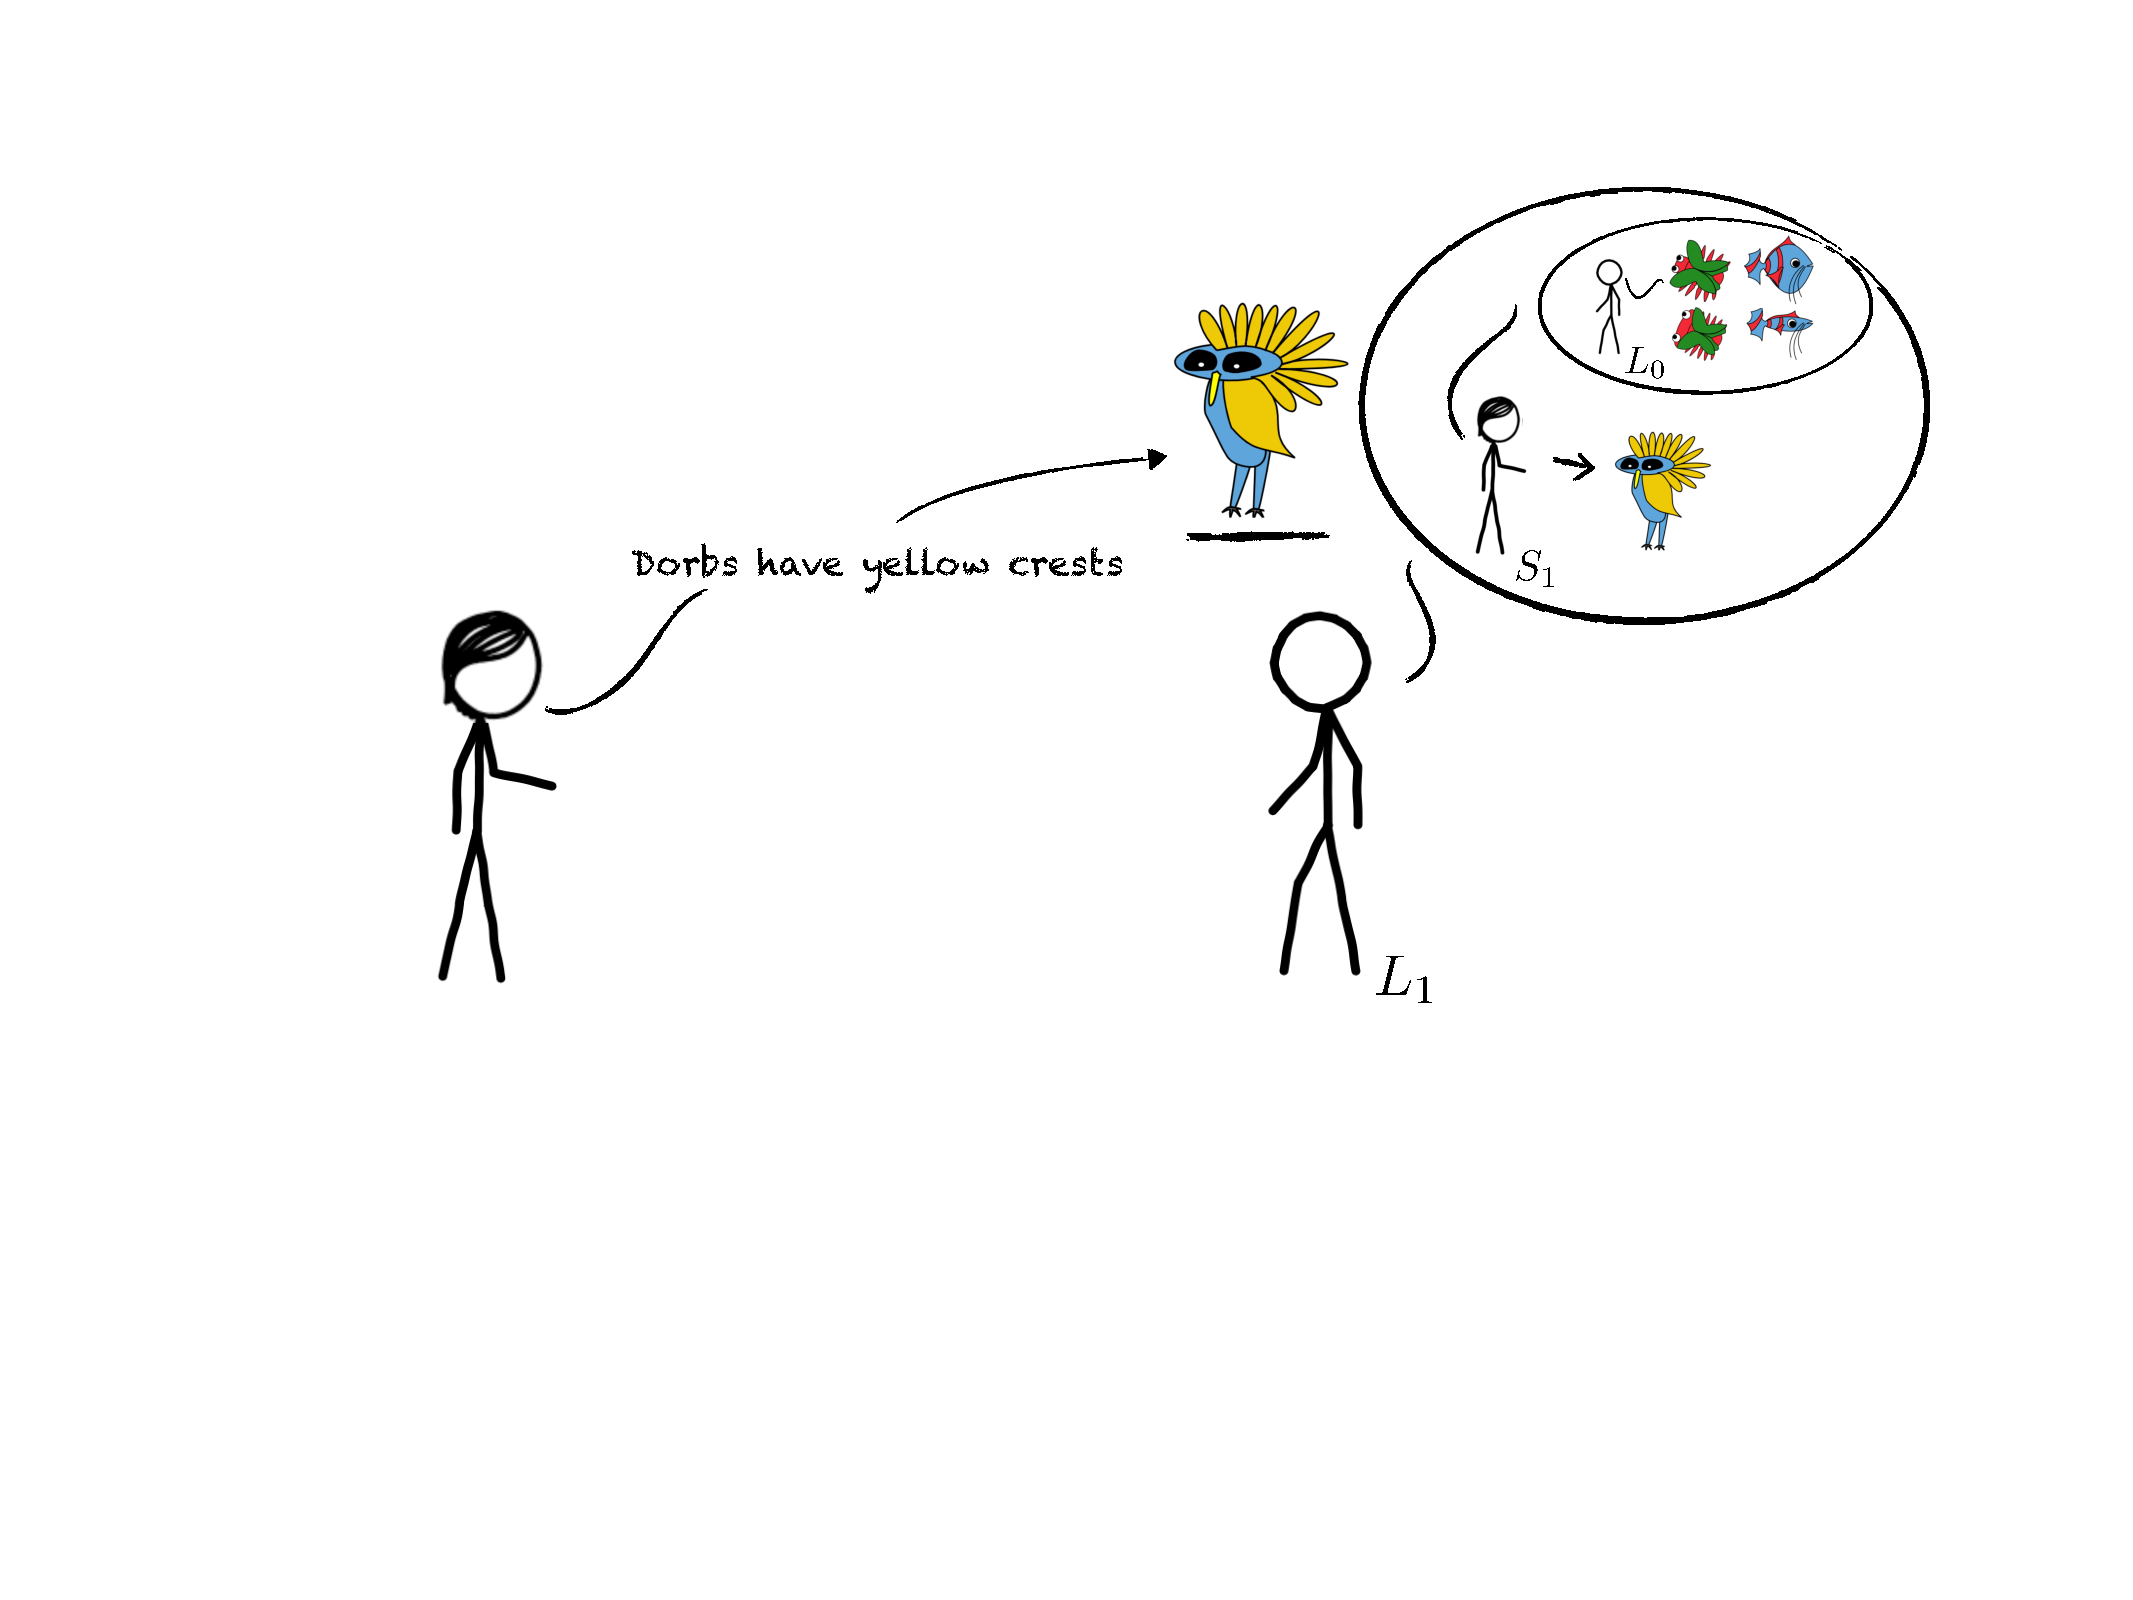
\includegraphics{figs/cartoon.pdf}
\caption{\label{fig:cartoon}Cartoon of the pragmatic generic interpretation model. The literal contribution of a generic (e.g., \enquote{Dorbs have yellow crests}) is equivalent to observing a single positive example (i.e., observing an actual dorb with a yellow crest). A pragmatic listener (\(L_1\)) interprets the utterance as coming from a speaker (\(S_1\)) who intentionally produced the utterance in order to convey information to a naive listener (\(L_0\)). The literal listener interprets the utterance by drawing on their prior knowledge about other categories and properties.}
\end{figure}

\hypertarget{computational-model}{%
\section{Computational Model}\label{computational-model}}

Generic language conveys generalizations about categories by predicating a property $f$ of a category $k$ (Carlson, 1977; Leslie, 2008).
Human generalization from observational data can be well described using the language of probability (Shepard, 1987) and Bayesian belief-updating with structured, prior knowledge (Tenenbaum et al., 2011).
We propose a null hypothesis that generics convey the same information-content as a single, positive observation interpreted with respect to structured background knowledge.
Formally, if a listener integrates their prior knowledge about the underlying probability or prevalence of the property---$P(f \mid k)$, denoted by \(r \in [0, 1]\)---with a single positive observation according to Bayes' rule, the model is:

%\begin{align}
%L_0(r, \mid u = gen) &= \frac{P(u = gen \mid r) \cdot P(r)}{\int_0^1 {P(u = gen \mid r') \cdot P(r') \mathop{}\!\mathrm{d}r'}}  \nonumber \\
% &= \frac{P(x = 1 \mid n = 1; r) \cdot P(r)}{\int_0^1 {P(x = 1 \mid n = 1; r') \cdot P(r') \mathop{}\!\mathrm{d}r'}}  \nonumber \\
% &= \frac{r \cdot P(r)}{\int_0^1 {r' \cdot P(r') \mathop{}\!\mathrm{d}r'}} \label{eq:L0}
%\end{align}

\begin{align}
L_0(r, \mid u = u_{gen}) &\propto P(u = u_{gen} \mid r) \cdot P(r)  \nonumber \\
 &= P(x = 1 \mid n = 1; r) \cdot P(r) \nonumber \\
 &= r \cdot P(r) \label{eq:L0}
\end{align}

\noindent where \(x\) denotes the number of positive examples and \(n\) denotes the number of observed examples, which are both equal to 1.
We take the conditional probability of the generic utterance \(u\) given some prevalence \(r\)---\(P(u\mid r)\)---to represent the literal semantic content of the generic utterance (Frank \& Goodman, 2012), which we define to be belief-updating from a single positive observation: \(P(x =1 \mid n = 1; r)\).
The latter is simply the probability of a coin with weight \(r\) landing on hands once, given that was flipped once, which is simply \(r\).
Given uniform prior beliefs about $r$ (i.e., all prevalence levels are equally likely \emph{a priori}), belief updating based on a single positive observation produces a posterior distribution that favors higher values of $r$ in proportion to their value (Figure~\ref{fig:tripartite}A, top panel). 
This model is mathematically equivalent to the interpretation model in Tessler and Goodman (2019), wherein generics update beliefs according to an uncertain threshold function (Appendix A).

\subsection{Prevalence priors}

According to this model of literal generic interpretation (Equation \ref{eq:L0}), the derivation of a literal interpretation of a generic balances the prior probability of different prevalence levels \(P(r)\) with the overall preference for higher prevalence levels \(r\) which results from observing a positive example.
The prevalence prior \(P(r)\) is a probabilistic representation of intuitive beliefs about properties and may display interesting structure reflecting these beliefs.
The distribution can also be understood as a distribution over different categories (and their associated prevalence of the feature).
For instance, a biological property (e.g., \emph{Xs fly}) manifests in many categories with 0\% prevalence (e.g., 0\% of dogs, rabbits, etc\ldots{} \emph{fly}); however, the property is present in other categories in very high proportions (robins, falcons, pterodactyls, etc\ldots{}); hence the distribution would have at least two modes: one around 0\% and another near 100\% (Figure~\ref{fig:tripartite}A second row).\footnote{
	We assume that people have graded degrees of belief and hence the mode at 0\% is not the same as a Delta distribution at exactly 0\%. Bayesians in general do not like to assign 0 probabilities to outcomes, which is what a mode at 0\% would entail for this cognitive model. Instead, the model assigns some very low but non-zero probability an instance of a category having a property which is not in general true of the category  (e.g., a dog flying), because it is not impossible to imagine some intuitive chain of causal events that could give rise to the property (e.g., a genetic mutation or a cross-species cloning experiment). 
}
A reproductive property like \emph{laying eggs} can manifest in only one sex of a category, which results in an intuitive distribution with a different bimodal structure.  
Finally, some properties may be expected to be present in only a minority of the category (e.g., because of a weak causal connection between the property and the kind such as \emph{carries malaria}; cf., Prasada, Khemlani, Leslie, \& Glucksberg, 2013) which would follow a different distribution as well (Figure \ref{fig:tripartite}A). 
Belief updating based on a single positive observation produces posterior distributions that are radically different depending on the prevalence prior distribution  (Figure \ref{fig:tripartite}A solid lines).
In our experiments, we both measure the prevalence priors for familiar properties  (Expt.~1) and manipulate the prevalence prior for an unfamiliar property (Expt.~2) in order to test the fine-grained quantitative influence of the prevalence prior on the implied prevalence of a generic statement. 


%Figure~\ref{fig:modelSimulations}A shows hypothetical prevalence priors for the features \emph{fly}, \emph{lay eggs}, and \emph{carry malaria} as well as an abstract property \emph{Y} without structured background knowledge.
%
%In a more abstract sense, the prevalence prior reflects beliefs about kinds and properties (e.g., there is something internal or external to the entity which causes it to have the property; cf., Prasada, Khemlani, Leslie, \& Glucksberg, 2013); if such a causal mechanism is believed to exist for some kinds and not others, we would expect the prevalence prior distribution to follow a mixture distribution (e.g., a mixture of Beta distributions as is shown for the \emph{fly}, \emph{lay eggs}, and \emph{carry malaria} cases above).\footnote{This assumption is similar in spirit to that employed by \emph{Hurdle Models} of epidemiological data, where the observed count of zeros is often substantially greater than one would expect from standard models, such as the Poisson (e.g., when modeling adverse reactions to vaccines; Rose, Martin, Wannemuehler, \& Plikaytis, 2006)}
%Such a structured prior distribution could vary by the mixture component (e.g., for how many different kinds does the mechanism exist?) as well as for the parameters of the component(s) that govern the prevalence for the kinds with the mechanism (i.e., given that there is such a mechanism, how strong do we expect that mechanism to be and do we expect further distinctions among those with a causal mechanism?).
%In the following simulations, we assume some mixture distribution structure.
%
%Interpretations from the literal generic interpretation model (Figure~\ref{fig:modelSimulations}B) can be understood as similar to different quantified statements (e.g., \emph{some} or \emph{most}) depending on the property. 
%For a biological property, a generic (\enquote{Xs fly}) is interpreted most similarly to \enquote{Most Xs fly}.
%This results from the prior distribution over a biological property like \emph{fly} being bimodal with modes near 0\% and 100\%.
%For the accidental property prior, \enquote{Xs carry malaria} is most similar to \enquote{Some Xs carry malaria} because the property is expected to be rare within categories in which the property is present.
%If a listener knows the existence of the property depends upon the sex of the creature (e.g., \emph{lays eggs}), the prevalence interpretation from a generic (\enquote{Xs lay eggs}) should be roughly that 50\% of the Xs lay eggs (only the females).

\begin{figure}
\centering
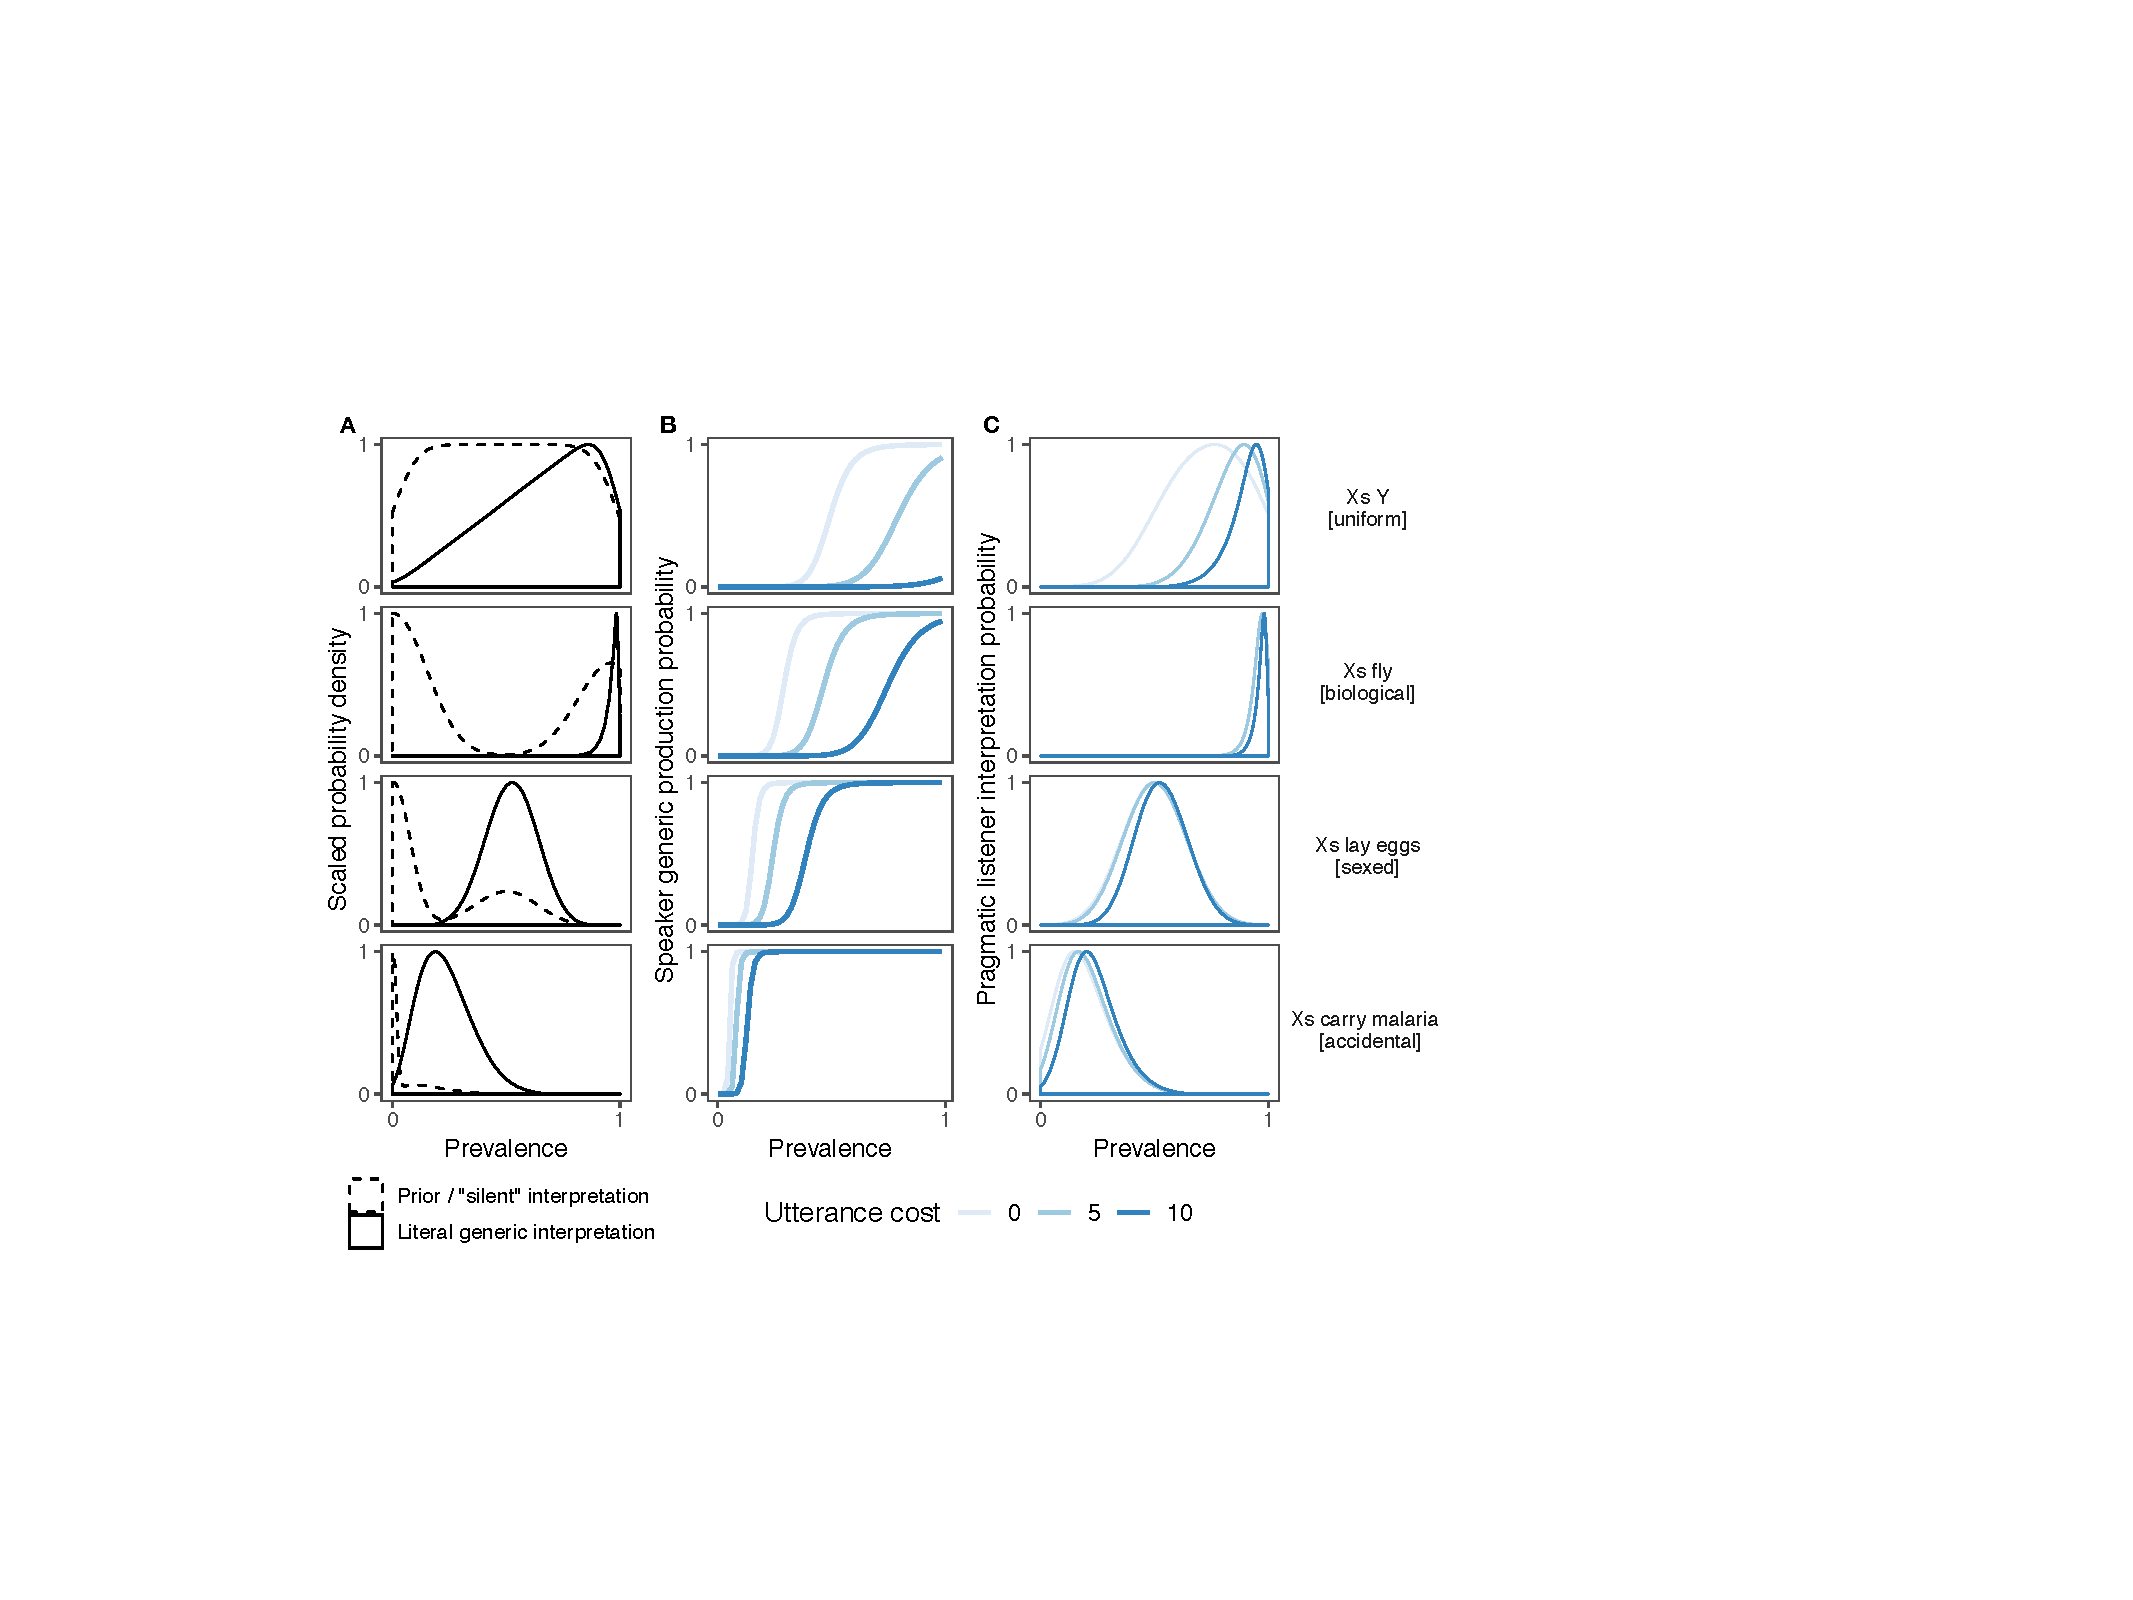
\includegraphics[width=0.8\textwidth]{figs/tripartite.pdf}
\vspace{0.5cm}
\caption{Examples of the three layers of the pragmatic interpretation model for four different properties. A: Literal listener $L_0$ interpretations (solid) for different prevalence priors (dashed). Priors also correspond to the literal interpretations of the ``silent'' utterance produced by the speaker $S_1$. B: Speaker $S_1$ production probabilities at different levels of prevalence for the generic utterance for three different costs of the generic utterance. C: Pragmatic listener interpretations of the generic utterance under different assumed costs of utterances. Differences between pragmatic and literal models are most pronounced for the priors with more uncertainty, such as the uniform prior. Speaker optimality parameter $\alpha$ set to 10 for panels B and C. Probability distributions are scaled so that the maximum density value in each panel is equal to 1. }
\label{fig:tripartite}
\end{figure}


\hypertarget{pragmatic-enrichment}{%
\subsection{Pragmatic enrichment}\label{pragmatic-enrichment}}



Even if the literal contribution of a generic sentence is informationally equivalent to observing a single, positive example, the inferences a listener derives from a generic could be meaningfully different from those one would glean from just a single example as the result of communicative reasoning  (Clark, 1996; Grice, 1975; Levinson, 2000).
Reasoning about why a speaker chooses to produce a generic could at the very least result in strengthened inferences, where the listener takes the generalization to apply more broadly than what a literal Bayesian reasoner would infer. 
%That is, a listener could reason about why the speaker choose to produce a generic utterance (when they could have stayed silent)
We model pragmatic reasoning by incorporating our model of a literal generic interpretation model (Eq.~\ref{eq:L0}) as a \emph{literal listener} model in the Rational Speech Act framework (Frank \& Goodman, 2012; Goodman \& Frank, 2016; Scontras, Tessler, \& Franke, 2018).
In such a model, a listener \(L_1\) interprets an utterance $u$ by reasoning about a speaker \(S_1\) intentionally producing the utterance to update the beliefs of the literal listener \(L_0\):

\begin{eqnarray}
S_1(u \mid r) &\propto& \exp{(\alpha \cdot \ln L_0(r \mid u) - \text{cost}(u))} \label{eq:S1} \\
L_1(r, \mid u) &\propto& S_1(u \mid r) \cdot P(r) \label{eq:L1}
\end{eqnarray}

Equation \ref{eq:S1} is a model of a softmax rational agent deciding whether or not to produce a generic utterance in order to convey information to a literal listener $L_0$  (Equation \ref{eq:L0}) taking into account the cost of producing the utterance.
The speaker makes this decision by choosing among their set of alternative utterances, which we assume only consists of producing the generic and staying silent: the act of silence produces a posterior distribution in the literal listener that is identical to the prior (Figure~\ref{fig:tripartite}A). 
Thus, choosing between a generic and silence amounts to how much more likely the speaker's personal level of prevalence $r$ (i.e., their belief about how many of the category have the property) is under the prior distribution over prevalence than under the posterior distribution given a single positive example, taking into account the cost of producing a statement (plausibly, \(\text{cost}(generic)\) \(>\) \(\text{cost}(silence)\)). 
This formulation results in speaker generic production probabilities that vary as a function of both their subjective prevalence of the feature, the prevalence prior, and the cost of the utterance (Figure~\ref{fig:tripartite}B).
This model was shown to be a good model of generic truth judgments (e.g., that ``Robins lay eggs'' is intuitively true, while ``Robins are female'' is not; why ``Sally runs'' is less felicitous than if Sally ran 3 times in the past year than if she ran 3 times in the past week; Tessler and Goodman, 2019) and we use it here for continuity with that work. 

Equation \ref{eq:L1} is a model of a pragmatic listener who understands that the generic utterance was produced by an intentional speaker \(S_1\) (Figure \ref{fig:cartoon}).
Again, interpretations are strongly driven by the prevalence priors, but pragmatic reasoning allows the utterances to imply stronger generalizations because a speaker might not have bothered to produce the generic if the prevalence was not sufficiently high, especially if the speaker incurred some cost in producing the utterance (Figure \ref{fig:tripartite}C).
The differences between literal and pragmatic interpretations are most pronounced for priors with more uncertainty, such as the uniform prior. 
We design our items in Expt.~1 to elicit a wide range of implied prevalence ratings in order to have sufficient quantitative variability to tell the literal~vs.~pragmatic models apart.
%For purposes of quantitative modeling, we allow both the cost of the generic---\(\text{cost}(generic)\)---and the speaker's rationality parameter \(\alpha\) to be free parameters that we infer from the behavioral data.


%\hypertarget{the-influence-of-prevalence-priors-and-pragmatic-reasoning}{%
%\subsection{The influence of prevalence priors and pragmatic reasoning}\label{the-influence-of-prevalence-priors-and-pragmatic-reasoning}}


\begin{figure}
\centering
%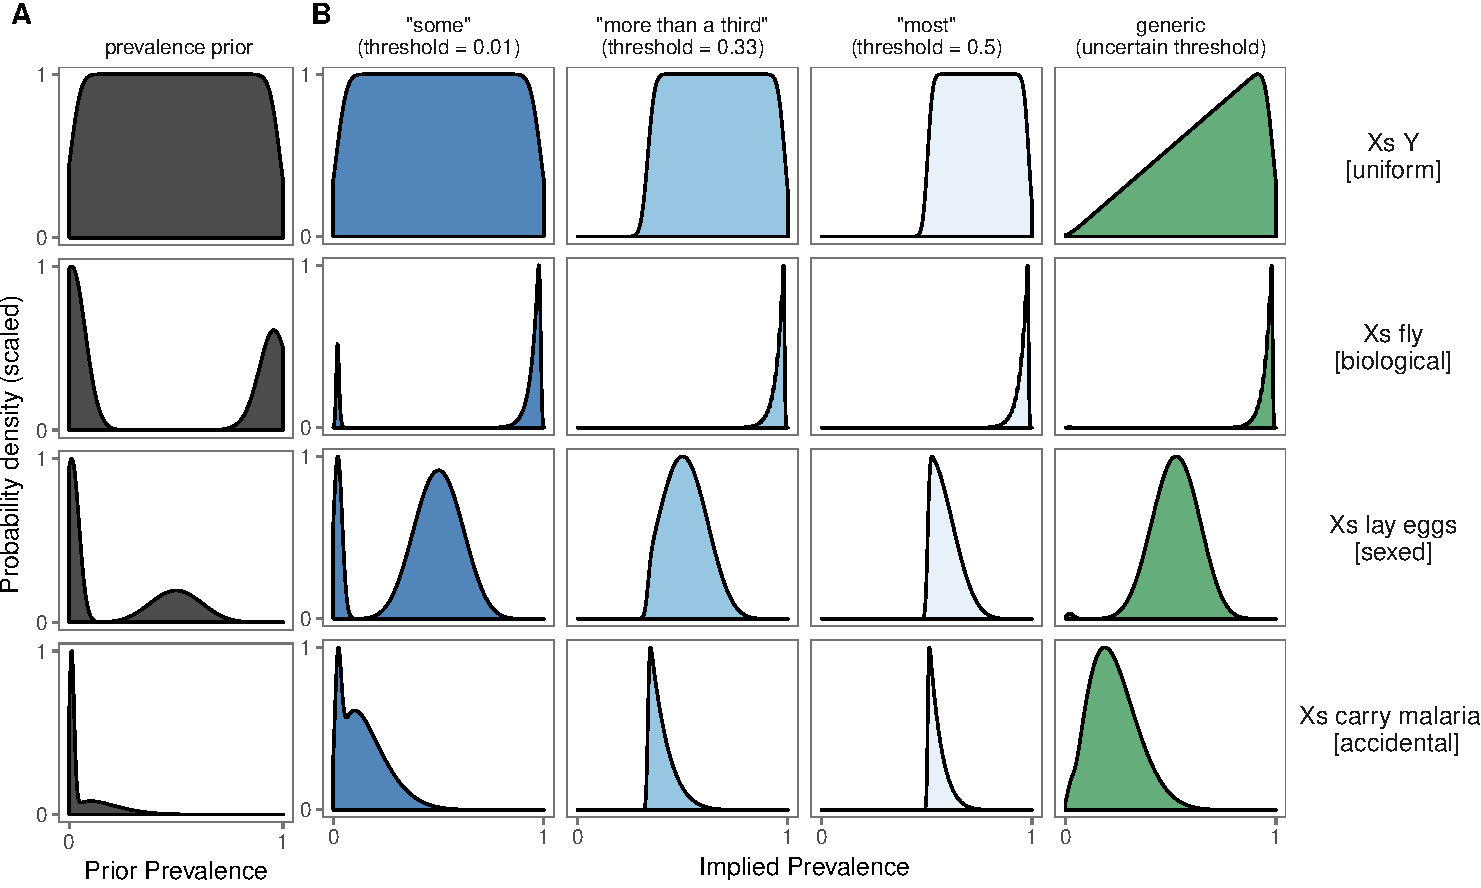
\includegraphics{genint_files/figure-latex/modelSimulations-1.pdf}
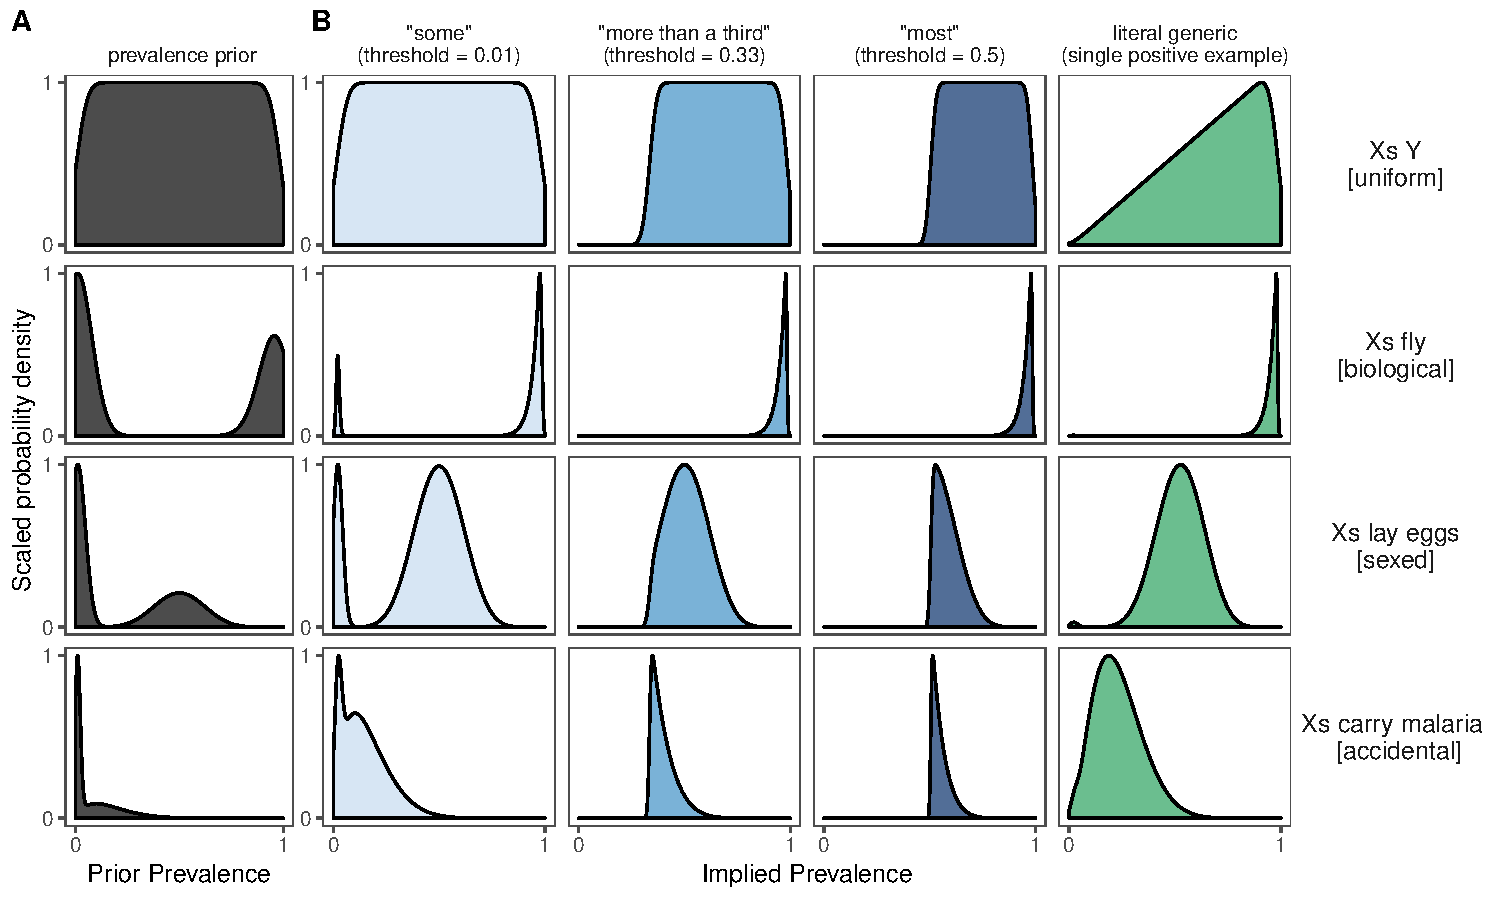
\includegraphics{figs/modelSimulations-noPrag.pdf}
\caption{\label{fig:modelSimulations}Comparison of literal generic interpretation to fixed-threshold models with various thresholds. A: Prevalence priors for four properties. B: Posterior distributions over prevalence (interpretations) given different belief updating rules: fixed-threshold quantifiers and the literal generic meaning as a single positive example.}
\end{figure}




%Interpreting a generic sentence as providing a single positive observation to the listener provides a way to understand generics in a highly property-specific manner.
%Listeners may derive a stronger interpretation of a generic, however, by reasoning about the communicative nature of the sentence they hear
%That is, a generic sentence is produced by a speaker who has the goal of conveying information to them.
%Figure~\ref{fig:tripartite} shows the predictions of each level of recursion in the pragmatic interpretation model (Eqs.~\ref{eq:L0}, \ref{eq:S1}, \ref{eq:L1}).
%The speaker model (Eq.~\ref{eq:S1})  decides to produce the generic by reasoning about whether to convey to the literal listener the distribution implied by the generic~vs.~the prevalence prior, which results from staying silent (or producing the ``null'' utterance; Figure~\ref{fig:tripartite}A).
%The speaker production probabilities thus strongly depend on the prevalence prior as well as the assumed cost of production (Figure~\ref{fig:tripartite}B).
%The pragmatic listener reasons that a speaker would only produce the generic at relatively high prevalence levels (\emph{relative} to the prevalence prior) and thus the fact that the speaker bothered to say the generic implies even higher prevalence than the literal meaning implies. 
%This inference is strengthened as the cost of the utterance increases, though in a way that respects the prevalence prior (i.e., not all generics can imply 100\% prevalence, even given high cost to the utterance; Figure~\ref{fig:tripartite}C).

%When learning about an abstract property with a uniform prevalence prior (top row), the pragmatic model infers more strongly that at least most of the category have the property.
%For the other prevalence priors, the pragmatic model predicts lower-variance interpretations.
%We design Experiment 1 with a diverse stimulus set to elicit a wide range of variability in interpretations that could distinguish the literal from the pragmatic generic interpretation models.

{\textcolor{Green}{[ndg: note: i changed "context" to other things (eg "property") in a bunch of places because what we're talking about is differences in target property and it's corresponding background knowledge. this is context in some sense, but i worry it would confuse people with more pragmatic / situated notions of context.]}}




\hypertarget{alternative-semantic-models}{%
\subsection{Alternative semantic models}\label{alternative-semantic-models}}

Both the literal and the pragmatic generic interpretation models treat the literal meaning of a generic as equivalent to observing a single minimal example from the category.
We compare these to alternative models that update beliefs according to a different literal meaning for the generic.
This comparison allows us to better understand how model predictions are influenced by the precise specification of a literal meaning.
In order to permit this comparison, we construct the alternative models with the same background knowledge in the form of the prevalence prior distribution \(P(r)\).
The alternative models take the literal meaning of a generic to be a fixed-threshold function, corresponding to models of quantifier semantics.\footnote{Note that a full model of quantifier interpretation would include their pragmatic interpretations (e.g., that \enquote{some} often implies \enquote{not all}). Such a model can be implemented in the same probabilistic modeling framework (Goodman \& Stuhlmüller, 2013) but does not directly address our question of whether a fixed-threshold semantics is tenable for generics.}
The first is a model of the quantifier \enquote{some} which rules out the lowest possible prevalence level:

\begin{eqnarray}
L_0^{some}(r \mid u) &\propto&  P(r \mid r > 0)  \label{eq:someModel}
\end{eqnarray}

The second is analogous to \enquote{most}, with a threshold at 50\% prevalence:

\begin{eqnarray}
L_0^{most}(r \mid u) &\propto&  P(r \mid r > 0.5)  \label{eq:mostModel}
\end{eqnarray}
Predictions of these control models are shown in Figure~\ref{fig:modelSimulations}.
A model that assumes a fixed threshold at 50\% is a very restricted model; it places zero probability on any response less than 50\%.
In case there are ratings in the experimental data sets that are less than 50\%, we must supplement the \enquote{most} model with an extrinsic noise process in order for this model to actually generate predictions for those data; that is, with some probability, participants respond at random.
We infer this noise probability parameter for the \enquote{most} model from the data.
Finally, we will compare the generic interpretation models to a model that does not update beliefs and predicts prevalence ratings according to the prior distribution \(P(r)\).
This comparison informs us as to whether or not participants actually \emph{update} their beliefs based on the generic statement.


\hypertarget{overview-of-experiments}{%
\section{Overview of Experiments}\label{overview-of-experiments}}

Our models of generic interpretation predict that the interpretations of generics in terms of prevalence should vary as a function of the prevalence prior.
Cimpian et al. (2010) found a difference in the implied prevalence between biological properties described with color adjectives (e.g., \emph{yellow fur}) and accidental properties (e.g., \emph{fungus-covered claws}).
We begin our experiments by first replicating and extending this result; this study serves to validate our measurement, which we will use in our main two experiments.
Experiment 1 is a larger scale version of Cimpian et al. (2010)\enquote{s \emph{implied prevalence} task, with sufficient measurements on the by-item level to reveal graded, quantitative variability between generics; additionally, we measure participants} prior beliefs and compare our generic interpretation models and control models.
Experiment 2 is a test of the causal influence of prevalence priors on generic interpretation, in which we manipulate participants' subjective prevalence priors in 10 different between-participants conditions.
The sample size, exclusion criteria, and planned statistical contrasts for each study were pre-registered on the Open Science Framework.
All cognitive and Bayesian data analytic models were implemented in the probabilistic programming language WebPPL (Goodman \& Stuhlmüller, 2014).
All data, analysis scripts, models, and links to experiments can be found at \url{www.github.com/mhtess/generic-interpretation}.

\hypertarget{preliminary-study-replication-and-extension-of-cimpian-et-al.-2010}{%
\section{Preliminary Study: Replication and Extension of Cimpian et al. (2010)}\label{preliminary-study-replication-and-extension-of-cimpian-et-al.-2010}}

%\hypertarget{method}{%
%\subsection{Method}\label{method}}

\hypertarget{participants}{%
\subsection{Participants, procedure, and materials}\label{participants}}

We recruited 40 participants over Amazon's crowd-sourcing platform Mechanical Turk.
The experimental design is very similar to Cimpian et al. (2010), and we chose to have a sample size at least twice as large as the original study (original n=15).
All participants were native English speakers.
The experiment took about 5 minutes and participants were compensated \$0.60.

%\hypertarget{procedure-and-materials}{%
%\subsubsection{Procedure and materials}\label{procedure-and-materials}}

In order to get participants motivated to reason about novel kinds, they were told they were the resident zoologist of a team of scientists on a recently discovered island with many unknown animals; their task was to provide their expert opinion on questions about these animals.
Participants were supplied with a bare plural about a novel category (e.g., \enquote{Feps have yellow fur}) and asked to judge prevalence: \enquote{What percentage of feps do you think have yellow fur?}
Participants completed in randomized order 25 trials: 5 for each of the biological properties and 10 for the accidental.

\hypertarget{results-and-discussion}{%
\subsection{Results and discussion}\label{results-and-discussion}}

Interpreting a novel generic sentence \enquote{Ks have F} often has the possibility of being understood as a universal or near-universal claim (\emph{all or almost all Ks Fs)}.
Across our the forty items in this experiment, however, we observe a gradient in the implied prevalence ratings, mostly clustered by the type of property (Figure~\ref{fig:cimpian-modelingResults}A).
At the level of property type, Cimpian et al. (2010) found a difference between the implied prevalence of generics about biological parts described with color adjectives (e.g., \emph{purple feathers}) and accidental properties (e.g., \emph{fungus-covered claws});  we replicate this result and extend it to show further gradability among types of properties (Figure~\ref{fig:cimpian-modelingResults}B).

\begin{figure}
\centering
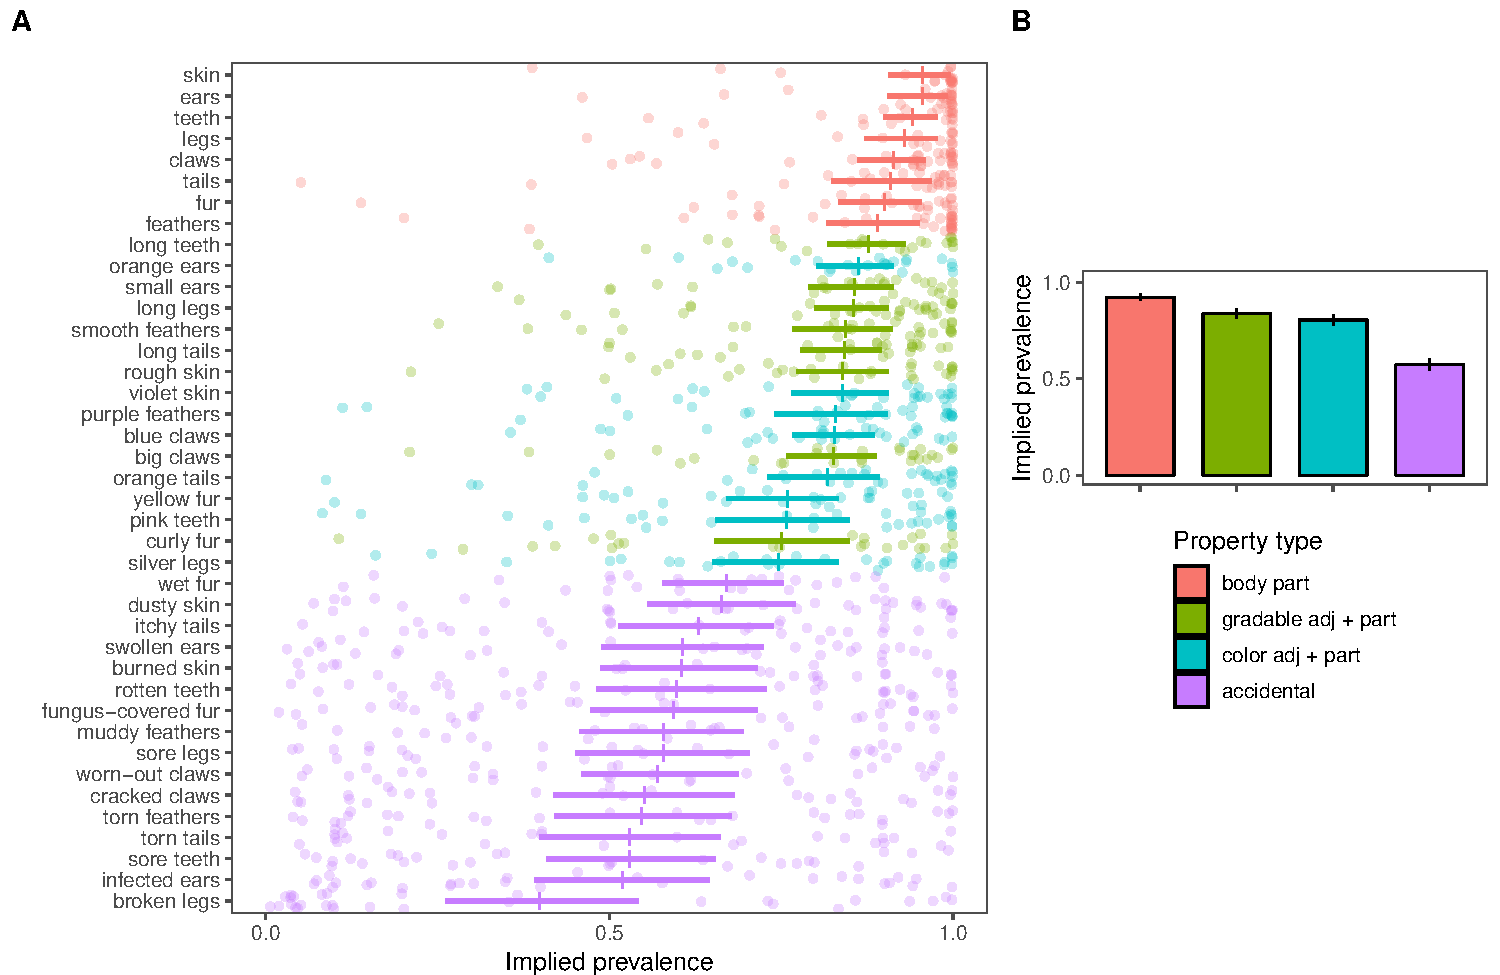
\includegraphics{figs/cimpian-results}
\caption{\label{fig:cimpian-modelingResults}Implied prevalence data for items from Cimpian et al. (2010). A: Implied prevalence ratings for forty body-part stimuli (\enquote{Ks have F}). Vertical line denotes mean, horizontal lines denotes bootstrapped 95\% confidence intervals, points are individual responses. B: Implied prevalence collapsed across property type. The original result of Cimpian et al. (2010) showed a difference between \emph{color adj + part} and \emph{accidental}.}
\end{figure}

Broadly, these results validate the measurement as one that can elicit variability, and it is this variability that is of primary concern to us.
The items that elicited the most variability in implied prevalence ratings were those of accidental or diseased states (e.g., \enquote{Lorches have broken legs}, \enquote{Wugs have fungus-covered claws}).
As Cimpian et al. (2010) noted, \enquote{properties of this type do not lend themselves very well to generic predication (Cimpian \& Markman, 2008; Gelman, 1988), so generics about broken legs, itchy skin, etc. are infrequent outside the laboratory.} (p.1472)
Not only are these kinds of statements infrequent outside the laboratory, bare plurals about accidental or diseased states (\enquote{Lorches have broken legs}) can easily be interpreted as non-generic, existential claims about the here-and-now, analogous to how \enquote{Dogs are on my front lawn} describes a particular state of affairs as opposed to something generalizable about dogs.
Since the strongest test of our models of generic interpretation will come from having to predict variability in implied prevalence ratings, we aim to elicit high variability in Experiment 1 using naturalistic properties that more easily lend themselves to generic predication (i.e., you could imagine a speaker saying the sentence).



\hypertarget{experiment-1}{%
\section{Experiment 1}\label{experiment-1}}

This experiment is designed to measure the prevalence implied by a generic about a diverse set of properties (Expt. 1b).
In addition, we first elicit participants' beliefs about the likely prevalence levels expected for these different properties (Expt. 1a).
We then use the elicited prevalence priors in our computational models and alternative models to make predictions about the prevalence implied by a generic.

\hypertarget{experiment-1a-prevalence-prior-elicitation}{%
\subsection{Experiment 1a: Prevalence prior elicitation}\label{experiment-1a-prevalence-prior-elicitation}}

In this experiment, we elicit prevalence knowledge about a diverse set of familiar properties.
Because the properties are relatively familiar, we elicit participants' knowledge by asking about the prevalence of the property among familiar categories.

\hypertarget{methods}{%
\subsubsection{Methods}\label{methods}}

\hypertarget{participants-1}{%
\paragraph{Participants}\label{participants-1}}

We recruited 200 participants from MTurk.
This number was arrived at with the intention of getting approximately 23 independent sets of ratings for each unique item in the experiment.
Participants were restricted to those with U.S. IP addresses and with at least a 95\% MTurk work approval rating (these same criteria apply to all experiments reported).
The experiment took on average 7.40 minutes and participants were compensated \$0.80.

\hypertarget{materials}{%
\paragraph{Materials}\label{materials}}

We created a stimulus set composed of seventy-five properties.
Items were generated by the first author by considering eight different classes of properties: physical characteristics (e.g., \emph{have brown spots}, \emph{have four legs}), psychological characteristics (e.g., \emph{experience emotions}), dietary habits (e.g., \emph{eat human food}), habitat (e.g., \emph{live in zoos}), disease (e.g., \emph{get cancer}, \emph{carry malaria}), reproductive behavior (e.g., \emph{have a menstrual cycle}), aggressive behaviors (e.g., \emph{pound their chests to display dominance}, \emph{hunt other animals}), and other miscellaneous behaviors (e.g., \emph{perform in the circus}, \emph{sing beautiful songs}); online sources about strange animal behaviors were consulted in order to find the more obscure properties. Full list of materials can be found in Table 4 in the Appendix.

\hypertarget{procedure-and-materials-1}{%
\paragraph{Procedure and materials}\label{procedure-and-materials-1}}

On the first trial, participants were asked to list three kinds of animals for each of five different classes of animals: mammals, fish, birds, insects/bugs, amphibians/reptiles.
The five classes of animals were presented in a randomized order on the screen and there were three text boxes for each in which participants could type an animal kind.
On subsequent trials, participants were shown a random subset of five animal kinds and asked what percentage each of these categories they believed had a property (e.g., \enquote{Out of all of the cheetahs in the world, what percentage do you think attack hikers?}).
Pilot results indicated similar responses were generated by a question about frequency (e.g., \enquote{Out of 100 cheetahs, how many do you think attack hikers?}).
Participants responded using a slider bar with endpoints labeled 0\% and 100\%, and the exact number corresponding to their slider bar rating was displayed once participants clicked on the slider bar.
Each participant saw a random selection of twelve properties.

As an attention check, at the end of the prior elicitation trials, participants were asked to select, from a list of ten, all of the properties they could remember being tested on.
The list included five properties that they had been tested on and five distractors.

\hypertarget{results}{%
\subsubsection{Results}\label{results}}

We used the same exclusion criteria that were preregistered for the subsequent generic interpretation study (Expt.~1b): \url{https://osf.io/bwn4t/register/5771ca429ad5a1020de2872e}.
Participants who did not have at least 4 out of 5 hits and at least 4 out of 5 correct rejections during the memory trial were excluded (\(n = 15\)).
In addition, we excluded participants who self-reported a native language other than English (\(n = 13\)).
This left a total of \(n = 175\) participants, with items receiving on average 28 (range = {[}16, 38{]}) unique participants responses (each participant provides five ratings).

A response in this task can be thought of as a sample from a property's prevalence prior distribution.
Thus, the distribution of responses for an item are an estimate of the prevalence prior distribution.
Figure~\ref{fig:genInt-prevPrior}A shows eight example items' distributions of responses.
For example, the property \emph{have four legs} is most likely either completely present (prevalence = 100\%) or completely absent (prevalence = 0\%) from categories.
\emph{Eat insects} looks similar, though there is considerable probability mass spread among the non-binary alternatives (\(0\% <\) prevalence \(< 100\%\)).
\emph{Get in fights with other animals} is similar but has substantially less probability mass at 100\% prevalence: It is unlikely that this property is widespread in a category.
\emph{Live in urban areas} shows a monotonically decreasing probability function; the higher the prevalence, the less likely it is.
\emph{Live in zoos} is expected to be even less prevalent, and the property \emph{has seizures} is expected to not be widespread at all.
The property \emph{get erections} is only expected to be present in 50\% of the population (presumably, the males) when it is present at all.

Most of the elicited prevalence prior distributions are at least bi-modal.
To visualize all properties simultaneously, we represent each distribution by two statistics: the relative probability mass at 0\%---\(P(\text{feature is present})\), or \(P(r > 0)\)---and the expected value (mean) of the distribution conditional on the prevalence being greater than 0\%---\(\mathbb{E}[P(r \mid r>0)]\) or the property's \emph{prevalence when present}.
The $P(\text{feature is present})$ is a measure of the (inverse-)distinctiveness of the feature (i.e., among how many animal categories is the property expected to be present). 
\emph{Prevalence when present} is the average prevalence among the categories for which the property has non-zero prevalence. 
Figure~\ref{fig:genInt-prevPrior}B shows the distributions of these two parameters: The stimulus set covers a wide range of possible values of both of these parameters.
This suggests we have sampled items with priors that exhibit a lot of quantitative variability.
Given these priors, our model makes quantitative predictions about the prevalence implied by a novel generic sentence (e.g., \enquote{Lorches live in zoos}).

\begin{figure}
\centering
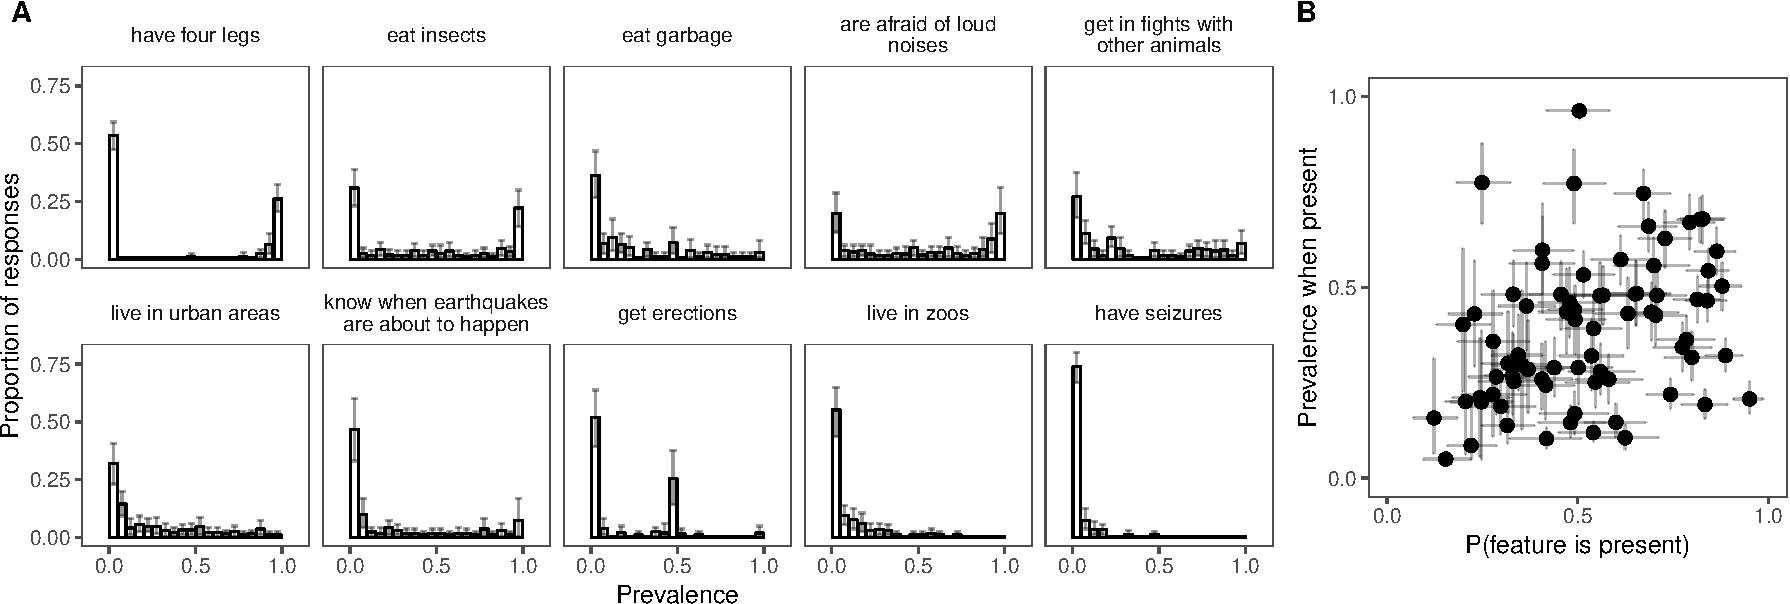
\includegraphics{genint_files/figure-latex/genInt-prevPrior-1.pdf}
\caption{\label{fig:genInt-prevPrior}Prevalence priors for a broad set of animal properties. A: Ten example prevalence priors elicited in Expt. 2a. Different prevalence priors give rise to different model predicted implied prevalence. B: Prevalence priors summarized by their relative probability mass at zero-prevalence P(feature is present), and their expected value among non-zero prevalence levels: Prevalence when present. The stimulus set covers a wide range of possible values of both of these parameters. Error bars denote bootstrapped 95\% confidence intervals.}
\end{figure}

\hypertarget{experiment-1b-generic-interpretation}{%
\subsection{Experiment 1b: Generic interpretation}\label{experiment-1b-generic-interpretation}}

\hypertarget{methods-1}{%
\subsubsection{Methods}\label{methods-1}}

\hypertarget{participants-2}{%
\paragraph{Participants}\label{participants-2}}

We recruited 200 participants from MTurk.
This number was arrived at with the intention of getting approximately 50 ratings for each unique item in the experiment.
The experiment took on average 5.50 minutes and participants were compensated \$0.80.

\hypertarget{procedure-and-materials-2}{%
\paragraph{Procedure and materials}\label{procedure-and-materials-2}}

The materials were the same as in Expt. 1a.
Participants were told that scientists had recently discovered lots of new animals that we did not know existed.
On each trial, they would be told facts about the new animals and be asked to translate it into the percentage of that animal it applies to.
On each trial, participants read \enquote{You are told: \emph{generic sentence}}, where the generic sentence was a bare plural statement about a familiar property \(F\) applying to a novel animal category \(K\) (e.g., \enquote{Javs attack hikers}).
They were then asked \enquote{Out of all of the \emph{K}s on the planet, what percentage do you think \emph{F}?} (e.g., \enquote{Out of all of the javs on the planet, what percentage do you think attack hikers?}).
Novel animal category names were mostly taken from Cimpian et al. (2010) and similar studies on generic language.
Participants responded using a slider bar with endpoints labeled 0\% and 100\%, and the exact number corresponding to their slider bar rating was displayed once participants clicked on the slider bar.
Each participant completed thirty-five trials, corresponding to a random subset of the full stimulus set.

After the generic interpretation trials, participants completed the same memory check trial as was done in the prior elicitation.
They were shown ten properties and asked to click on those they had seen in the experiment.
Following the memory check trials, participants completed up to five explanation trials, depending on their ratings in the task.
On an explanation trial, participants saw a rating they had given for a property they had rated as applying to less than 50\% and asked if they could explain why they gave the response that they gave.
Participants also had the option of changing their response after providing an explanation.
These data were only used in exploratory analyses and not for the main analyses reported below.
If participants gave no ratings less than 50\%, they did not complete any explanation trials.

\hypertarget{descriptive-results}{%
\subsubsection{Descriptive results}\label{descriptive-results}}

We used preregistered exclusion criteria, which were also used for Expt. 1a.
Participants who did not have at least 4 out of 5 hits and at least 4 out of 5 correct rejections during the memory trial were excluded (\(n = 62\)).
In addition, we excluded participants who self-reported a native language other than English (\(n = 8\)).
This left a total of \(n = 132\) participants, with items receiving on average 62 responses (range = {[}50, 77{]}).

As in the replication of Cimpian et al. (2010), we observe a clear gradient in the implied prevalence ratings across our seventy-five items (Figure~\ref{fig:genint-empiricalData}).
On one end of the continuum, there is a generic like \enquote{Wugs have four legs}, which is interpreted as a universal---applying to exactly 100\% of wugs---by 36 out of 70 participants and which received a mean implied prevalence rating of \(0.96 [0.93, 0.98]\).\footnote{Note the novel category term is randomized for each participant and property.
  We use particular novel category terms in the text for ease of exposition.}
On the other end is \enquote{Glippets perform in the circus}, which is interpreted as applying to less than 25\% of glippets by 35 out of 61 participants and which receives a mean rating below 50\% (\(0.31 [0.23, 0.39]\)).
Additionally remarkable is the distribution of responses for individual items: Though \enquote{Feps live in zoos} probably means around 25\% of feps live in zoos, it is still quite possible that almost 100\% live in zoos (e.g., in the real world, 100\% of Micronesian Kingfishers live in zoos).

To assess the reliability of these data, we ran a replication (\(n=140\)) using a slightly different dependent measure.\footnote{By experimenter error, only seventy-four of the seventy-five items were collected in the replication data set.}
Instead of being asked a question about percentages (e.g., \enquote{Out of all of the Ks in the world, what percentage F?}), participants were asked a question in terms of frequency: \enquote{Out of 100 Ks, how many do you think F?}.
The empirical by-item means between these data and the original data are highly correlated (\(r(74) = 0.96\), \(r_{spearman}(74)= 0.96\)), indicating very high data reliability.

\begin{figure}
\centering
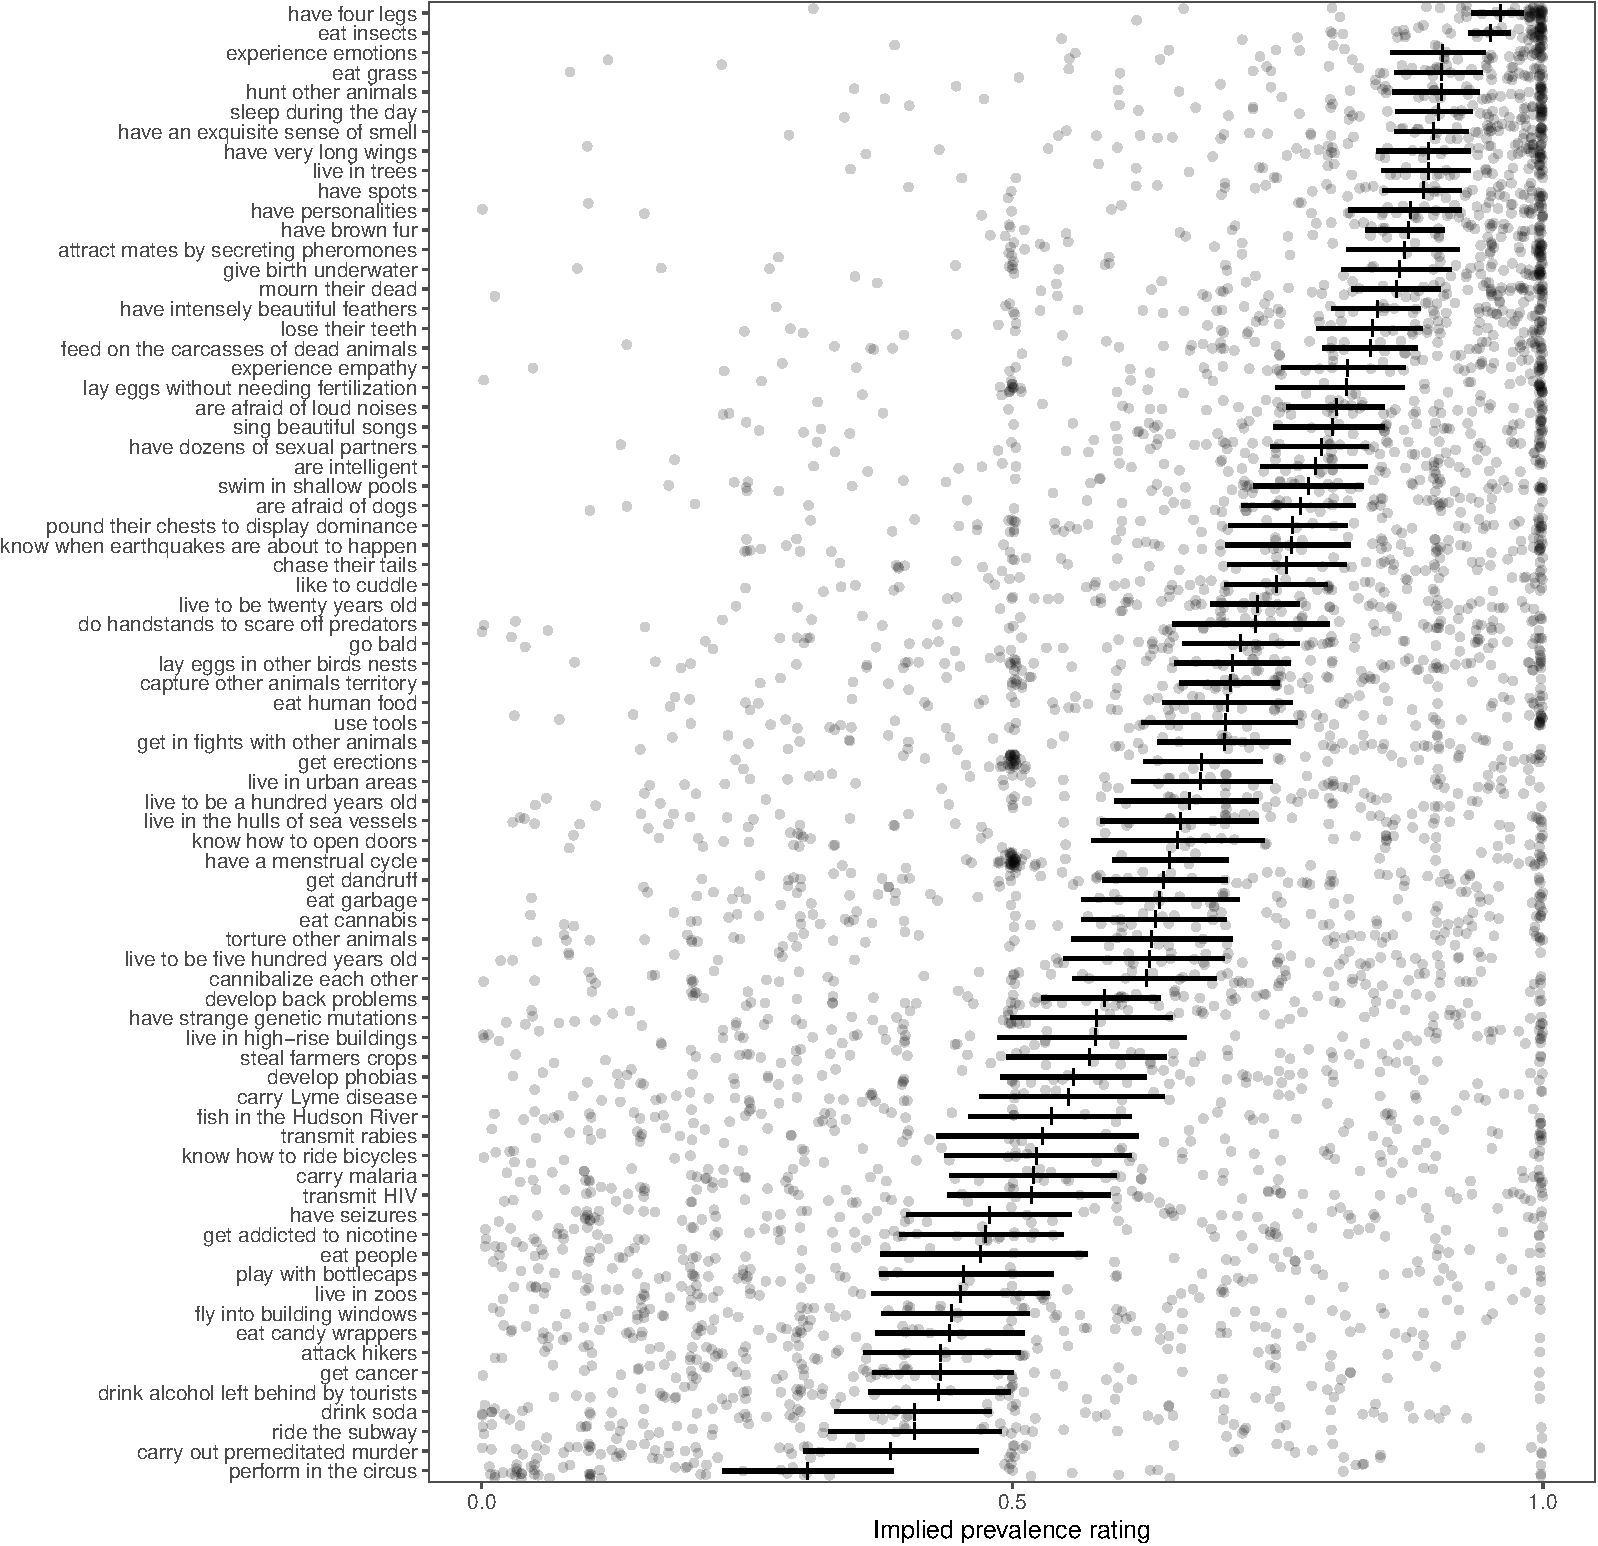
\includegraphics{genint_files/figure-latex/genint-empiricalData-1.pdf}
\caption{\label{fig:genint-empiricalData}Implied prevalence ratings for a diverse set of seventy-five items. Vertical lines denote means, points are individual empirical judgments. Error bars denote bootstrapped 95\% confidence intervals.}
\end{figure}


\hypertarget{model-based-analyses}{%
\subsubsection{Model-based analyses}\label{model-based-analyses}}

Our model-based analyses ask how well the various semantics models accommodate the human generic interpretation data and which model provides the most parsimonous view of the data.
We estimate various model parameters using Bayesian methods in order to determine the most likely values of the latent parameters given our hypotheses about how the both the prior elicitation and generic interpretation data were generated.\footnote{Appendix C in Tessler and Goodman (2019) provides a careful analysis of the behavior of this joint Bayesian inference strategy for jointly modeling the prevalence prior parameters together with other parameters of the model governing generic interpretation. They find imperceptibly small differences between the parameters inferred from the prevalence prior data in isolation and those inferred by jointly modeling the prior elicitation together and the generic interpretation data, suggesting that the prevalence priors are not significantly distorted by this method in order to provide a stronger quantitative fit to the generic interpretation data.}
That is, we ask if there is some reasonable setting of the prevalence priors that, together with a particular model of generic interpretation, could give rise to the generic interpretation results.
We also compare the generic interpretation models to each other and a number of control models using the standard Bayesian model comparison metric: marginal likelihoods, or Bayes factors.

We posit uncertainty in the parameters governing the listener prevalence prior distribution.
Our prior elicitation task helps constrain the values of the parameters of the prevalence priors, which we assume takes the form of a three-component mixture of Beta distributions model.\footnote{We use Beta distributions to match the form of the response variable: a number between 0 - 1.}
The only other parameters we introduce are specific to certain generic interpretation models.
The model that assumes a literal semantics identical to the quantifier \enquote{most} (threshold at 0.5) must be outfitting with an extrinsic noise parameter in order to accommodate responses that are literally false under this interpretation of a generic (i.e., implied prevalence ratings below 0.5).
The pragmatic generic interpretation model posits that listeners interpret generics by strengthening a literal meaning equivalent to a single positive example of the category with the communicative force of an utterance produced by an intentional speaker.
This model thus has two additional free parameters: The implicit cost of producing a generic in comparison to staying silent (\emph{utterance cost}) and the degree of information-theoretic optimality with which the speaker behaves (\emph{speaker optimality}).
Comparing models using the marginal likelihood of the data will penalize the pragmatic model because of these additional degrees of freedom (Lee \& Wagenmakers, 2014).

\hypertarget{model-definition-and-inference}{%
\paragraph{Model definition and inference}\label{model-definition-and-inference}}

For each candidate model of generic interpretation (literal, pragmatic, \enquote{some}, \enquote{most}), we build a joint Bayesian data-analytic model to simultaneously predict the prevalence prior data (Expt. 1a) and the generic interpretation data (Expt. 1b), similar to the methods of Tessler and Goodman (2019).
We model the prevalence prior data as coming from a mixture of three Beta distributions and we model the generic interpretation data as being generated from the candidate computational model of generic interpretation.
Each prevalence prior has eight parameters governing its shape: a mean \(\gamma\) and variance parameter \(\xi\) for each of the three Beta components and two parameters \(\phi_1\), \(\phi_2\) that describe the relative weighting among the three components.
We put uninformative priors over these parameters \(\gamma \sim \text{Uniform}(0, 1)\), \(\xi \sim \text{Uniform}(0, 100)\), \(\phi \sim \text{Dirichlet}(1,1,1)\).\footnote{Another reasonable, less structured model of the prevalence prior data would be a Dirichlet over discretized bins along the prevalence scale. We choose the mixture-of-Betas formulation because it assumes some correlation between neighboring values along the scale and has fewer parameters. }
The inferred prevalence prior distributions are then used as the prevalence prior \(P(r)\) in whatever model of generic interpretation we are testing in order to generate predictions for the generic interpretation data.\footnote{Though described sequentially, this inference procedure is actually performed simultaneously.}
In addition, the model of \enquote{most} semantics has an additional noise parameter, which adds a probability \(\phi\) of a participant responding randomly; we put a uniform prior over the value of this parameter to estimate the proportion of responses this model would have to chalk up to noise in order to accommodate: \(\phi \sim \text{Uniform}(0, 1)\).
The pragmatic generic interpretation model (Eq. \ref{eq:L1}) has two free parameters : the rationality of the speaker model \(\alpha\) and the speaker's cost of producing the generic utterance (in comparison to staying silent) \(c = \text{cost}(generic)\), over which we put uninformative priors, consistent with the literature on this class of models: \(\alpha \sim \text{Uniform}(0, 30)\) and \(c \sim \text{Uniform}(0, 10)\).
The literal generic interpretation model and models of \enquote{some} and \enquote{most} quantifier semantics have no additional parameters.
To learn about the credible values of the parameters as well as generate model predictions for the generic interpretation data, we performed Bayesian inference on each model by running three chains of an incrementalized version of MCMC (Ritchie, Stuhlmüller, \& Goodman, 2016) for 750,000 iterations, removing the first 250,000 iterations for burn-in.
Convergence was checked qualitatively by confirming the similarity of the results across chains; there were no appreciable differences in the results between different chains.



\begin{figure}
\centering
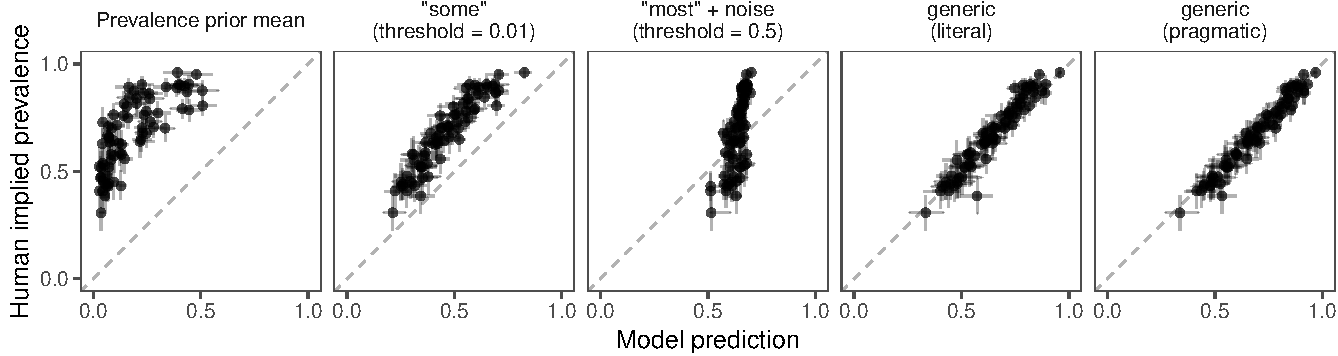
\includegraphics{genint_files/figure-latex/genint-modelingResults-1.pdf}
\caption{\label{fig:genint-modelingResults}Posterior predictive model fits for quantitative models based on (from left to right): (i) the mean of the prevalence prior, (ii) a threshold semantics fixed at 0.01 (\enquote{some}), (iii) a threshold semantics fixed at 0.5 (\enquote{most}), (iv) a single positive observation (literal generic), and (v) a pragmatically interpreted single positive observation (pragmatic generic). The model for \enquote{most} is outfitted with a noise parameter to accomodate data points that are logically impossible given the fixed semantics. Error bars denote bootstrapped 95\% confidence intervals for the behavioral data and 95\% highest posterior density intervals for the model predictions.}
\end{figure}

\hypertarget{model-criticism}{%
\paragraph{Model criticism}\label{model-criticism}}

{\textcolor{Green}{[ndg: we should have a brief result reporting the posterior predictive check on the priors data? ie how well does our joint data analysis accommodate the empirical patterns in the prevalence priors.]}}
{\textcolor{Blue}{[mht: this paragraph okay?]}}

A qualitative examination of the inferred prevalence prior distributions showed that they were well-modeled as a mixture of three Beta distributions.
Often one Beta distribution is devoted to accounting for the very small numbers (0\% or near 0\% prevalence ratings, for all the categories for which the property is absent), while the two other components account for the other parts of the distribution of responses, the details of which depend upon the property (see Figure~\ref{fig:genInt-prevPrior} for examples of priors of different shapes).
To provide a quantitative examination of the fit to the priors data, we look at the posterior predictive distribution discretized to bins in increments of 10\% prevalence (i.e., categorical distributions over the bins of 0\%, 10\%, \ldots{}, 90\%, 100\% prevalence) and compare the model's inferred priors to the empirical counts that fell into those bins in the prior elicitation task.
The joint data analysis model accommodates the empirical patterns in the prevalence priors very well: \(r^2(825) = 0.99\), \(MSE = 0.00052\).

To evaluate how well each model can accommodate the implied prevalence data, we compare the Maximum A-Posteriori value of each model's posterior predictive distribution of implied prevalence ratings to the mean implied prevalence ratings for each of the 75 items.
Table 1 shows the mean squared errors and proportion of explained variance for predictions based on the prevalence prior alone, a literal \enquote{some} model, a literal \enquote{most} model (which includes an additional fit noise parameter), a literal generics model (single positive observation), and the pragmatic generics model.
Figure~\ref{fig:genint-modelingResults} reveals that the models based on the prevalence prior and the quantifier \enquote{some} (i.e., a fixed threshold at the lowest possible value) consistently \emph{underpredict} the implied prevalence, consistent with the intuition that assigning the semantics of \enquote{some} for generics is too weak.
Though the model based on a semantics for \enquote{most} (i.e., a fixed threshold at 0.5) does better in terms of mean squared error, it explains substantially less variance; the \enquote{most} model assigns 0.57 {[}0.55, 0.59{]} proportion of the data to be noise, because of the high number of responses below 50\%.
Unlike each of the alternative semantic models, the two models based on belief updating according to a single, positive observation (literal and pragmatic generics models) can accommodate the highly variable generic interpretation data with a high degree of quantitative accuracy.
The pragmatic model slightly outperforms the literal generics model in terms of both mean squared error and variance explained at the level of average responses.
The inferred values of the speaker optimality parameter \(\alpha\) was 2.03 {[}1.82, 2.18{]} and the generic cost parameter \(c\) was 3.6 {[}3.16, 4.27{]}.

\begin{figure}
\centering
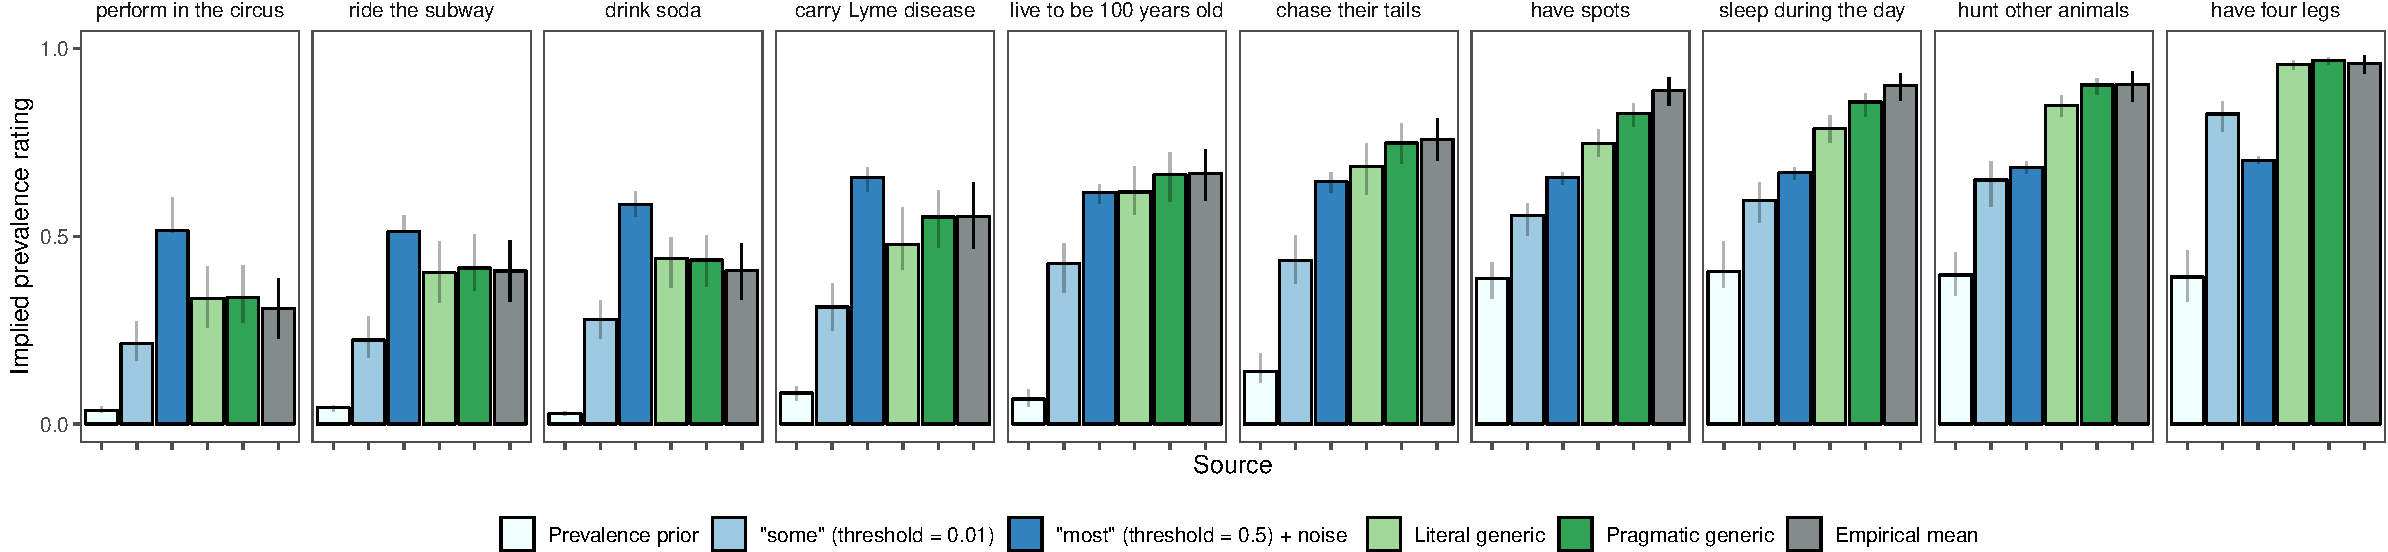
\includegraphics{genint_files/figure-latex/genint-modelingResults-bars-1.pdf}
\caption{Implied prevalence ratings and model predictions for eight items that cover the spectrum of prevalence ratings. 
Both generic models closely track the implied prevalence ratings, but the pragmatic model shows stronger interpretations for a number of important cases.}
\label{fig:genint-modelingResults-bars}
\end{figure}


Figure~\ref{fig:genint-modelingResults-bars} shows empirical means and model predictions for eight example items covering the range of average responses from roughly 30\% implied prevalence to almost 100\%.
All models exhibit some sensitivity to the variance in implied prevalence ratings, because they all have the prevalence prior in their definition.
It is the actual magnitude of the strength of the generalization implied by the utterance that is predicted to be different, with the prior and \enquote{some} models predicting too weak of an interpretation.
\enquote{Most} is handicapped by its high inferred rate of noise and does not make dramatically different predictions across the items.
Both the literal and pragmatic generic interpretation models track the quantitative variance across these items.
The evidence for pragmatic interpretations is most apparent for items that receive high but not at-ceiling implied prevalence ratings (e.g., \emph{have spots}, \emph{hunt other animals}; Figure~\ref{fig:genint-litPrag-scatter}), suggesting that interpretations are most in dangerous of being strengthened beyond a speaker's intent for properties for which the listener is most uncertain about their distribution (cf., the asymmetry reported in Cimpian et al., 2010).
{\textcolor{Blue}{[mht: could do a regression comparing whether or not the pragmatic model is better than the literal model (or the difference in sq.err) vs. the entropy of the prior... to see if pragmatics is most visible under conditions of uncertainty]}}




\begin{table}[h]
\centering
\begingroup\fontsize{10pt}{11pt}\selectfont
\begin{tabular}{llll}
  \hline
Model & MSE & $r^2$ & Log marginal likelihood \\ 
  \hline
Prior & 0.2578 & 0.578 & -18006 \\ 
  "Some" & 0.0479 & 0.879 & -15309 \\ 
  "Most" & 0.0213 & 0.491 & -13135 \\ 
  Literal Generic & 0.0026 & 0.933 & -12843 \\ 
  Pragmatic Generic & 0.0015 & 0.962 & -12781 \\ 
   \hline
\end{tabular}
\endgroup
\caption{Summary statistics for models of generic interpretation. Mean Squared Errors and variance explained are calculated at the level of the item averages. Marginal likelihood is computed over the full distribution of responses.} 
\end{table}

\begin{figure}
\centering 
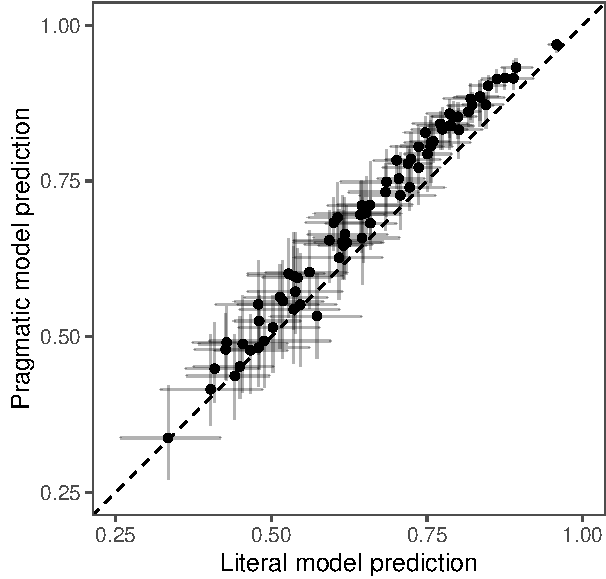
\includegraphics[width=0.4\textwidth]{genint_files/figure-latex/genint-litPrag-scatter-1} 
\caption{Comparison of implied prevalence predictions for the literal~vs.~pragmatic generic interpretation models. The pragmatic model shows stronger interpretations for items that have intermediate implied prevalence.}
\label{fig:genint-litPrag-scatter}
\end{figure}


\hypertarget{model-comparison}{%
\paragraph{Model comparison}\label{model-comparison}}

Our second data analytic strategy is a formal model comparison to determine the extent to which the pragmatic generic interpretation model is the best explanation of the data, given it is a slightly more complex model than the literal interpretation model.
To do this, we compute Bayes Factors which compare the likelihood of the observed data under each of the models, averaging across all values of the free parameters of a model.
This form of model comparisons penalizes models with extra free parameters if, in fact, the model's predictions are highly sensitive to exact values of those parameters.
Comparing our models using a fully Bayesian strategy with uncertainty over the prevalence priors (analogous to what is performed in the model criticism section) is computationally challenging.
Therefore, we compute the likelihood of the data under each model by fixing the prevalence priors to the raw empirical distributions; fixing the prevalence priors reduces the overall flexibility of the models, but does so in a way that penalizes all models to an equal extent.
To estimate the marginal likelihood of the data under each model, we used an Annealed Importance Sampling algorithm (Neal, 2001) implemented in the probabilistic programming language WebPPL.
The results are shown in Table 1: The pragmatic model is on the order of \(e^{60}\) times better at accounting for the implied prevalence data, even taking into the model's additional flexibility.
This is extremely strong evidence that the best model for how generics update beliefs is as a single positive example understood as being produced with a pedagogical intent.



\hypertarget{experiment-2-prior-manipulation}{%
\section{Experiment 2: Prior Manipulation}\label{experiment-2-prior-manipulation}}

In this experiment, we test the causal role of the prevalence prior in generic interpretation.
In the previous experiment, we saw how participants' prior beliefs about the prevalence of the property measured by asking about alternative categories (Expt. 1a) related to the prevalence implied by a novel generic (Expt. 1b) via the pragmatic generic interpretation model.
Though the pragmatic generics model is able to finely track interpretations in a way that alternative models cannot, the evidence so far for the influence of the prevalence prior on interpretation is merely correlational.
Here we manipulate the prevalence prior and measure the resulting influence on interpretation.
To serve as a manipulation check, we first elicit predictions about prevalences following our prior manipulation procedure; these predictions also serve as the measurements of the (manipulated) prevalence priors used in our model.

\hypertarget{experiment-2a-prior-elicitation-manipulation-check}{%
\subsection{Experiment 2a: Prior elicitation (manipulation check)}\label{experiment-2a-prior-elicitation-manipulation-check}}

\hypertarget{methods-2}{%
\subsubsection{Methods}\label{methods-2}}

\hypertarget{participants-3}{%
\paragraph{Participants}\label{participants-3}}

We recruited 200 participants from MTurk.
This number was arrived at with the intention of getting approximately 30 ratings for each unique item in the experiment.
The experiment took on average 3 minutes and participants were compensated \$0.30.

\hypertarget{materials-1}{%
\paragraph{Materials}\label{materials-1}}

The goal of this experiment was to manipulate the prevalence prior.
Participants were familiarized with one of ten prevalence prior distributions, shown in Figure~\ref{fig:priorManipulationExpt}E).
Nine of the ten distributions were bimodal with modes either at 0\%, 25\%, 50\%, 75\%, or 100\%; the tenth distribution was uniform over all prevalence levels between 0\% and 100\%.
The mixture between the two modes was always 50\% (half of samples were from one mode and half from the other, as shown in Figure~\ref{fig:priorManipulationExpt}B).

Our cover story involved learning about a single property (\emph{know when earthquakes are about to happen}).
We used this property because its prevalence prior elicited in Expt. 1a suggested participants had a lot of uncertainty as to what prevalence levels to expect for this property; we thus expected this property might be particularly amenable to manipulation.\footnote{Pilot testing using a completely novel property (e.g., \emph{daxing}) appeared to make the task too artificial. Participants seemed to treat the task as a number game. }

\hypertarget{procedure}{%
\paragraph{Procedure}\label{procedure}}

\begin{figure}
\centering
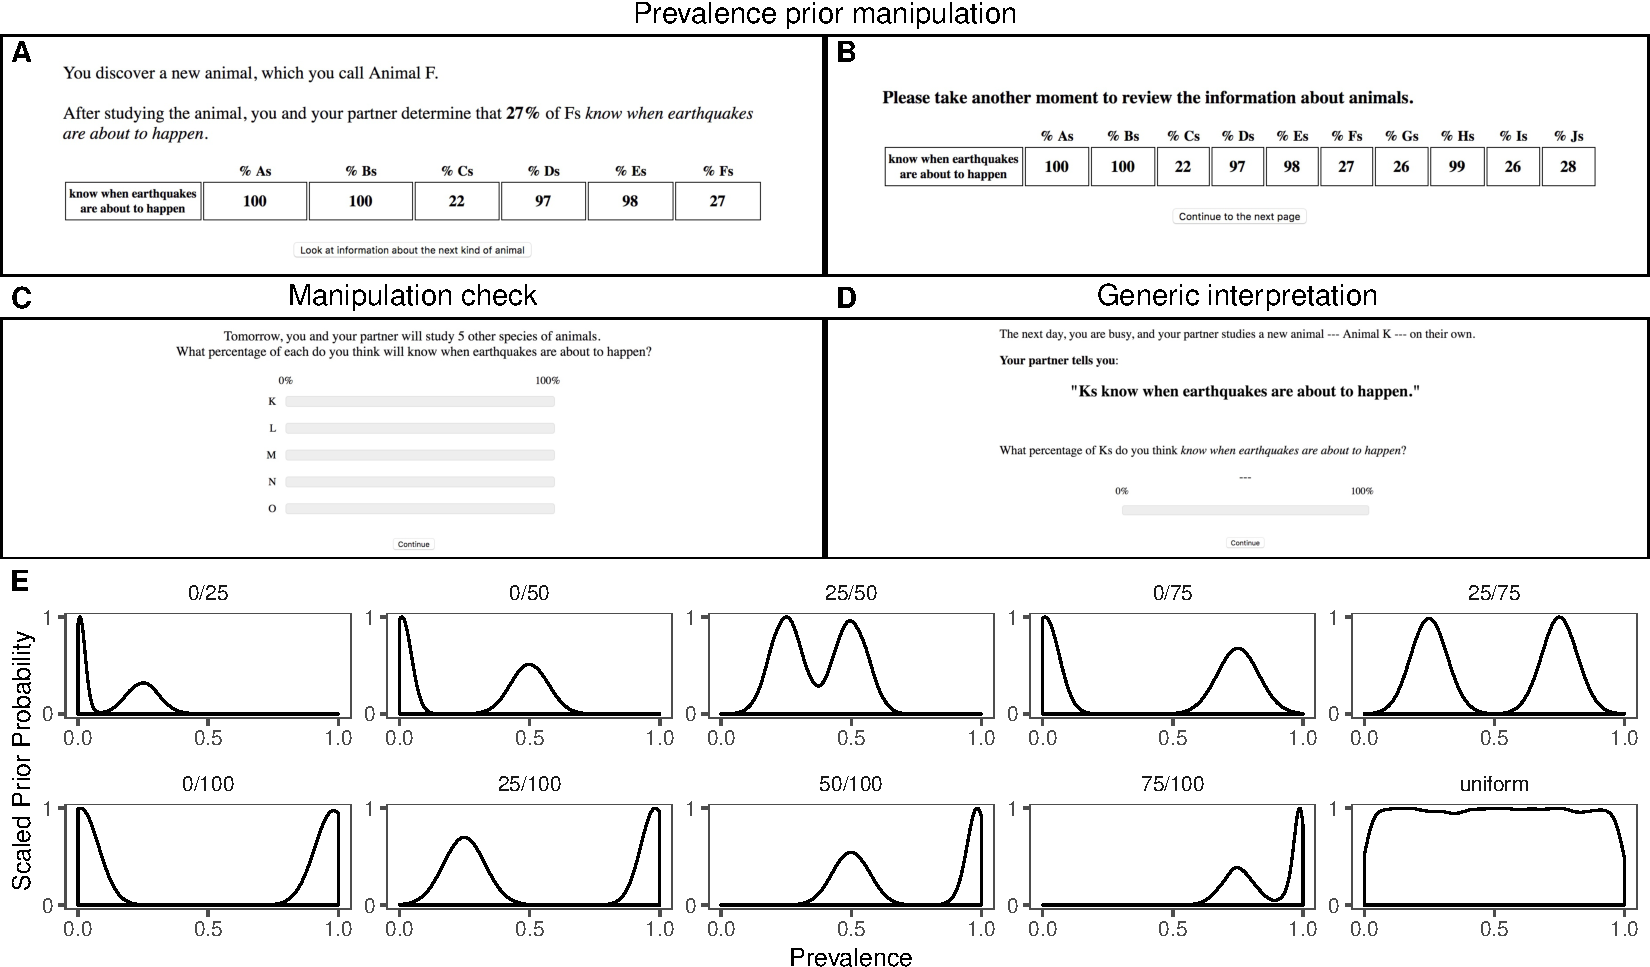
\includegraphics{genint_files/figure-latex/priorManipulationExpt-1.pdf}
\caption{\label{fig:priorManipulationExpt}Overview of Experiment 2. A: Prevalences of feature in animals are shown one at a time, described in text and displayed in a table. B: Participants are asked to review previous results once all displayed. C: Prior elicitation task: Participants predict the results of the next five animals. D: Generic interpretation task: Participants rate prevalence after reading generic sentence. E: Experimentally manipulated prevalence prior distributions. The distribution shown in B is the \emph{weak or deterministic} distribution.}
\end{figure}

In order to avoid participants learning the structure of the task, participants completed only a single trial: Each participant saw only one prevalence distribution.
Participants were given a cover story in which they were asked to imagine they were an astronaut-scientist exploring a distant planet with lots of new animals on it.
They were studying these animals with another scientist to understand the animals' ability to \enquote{know when earthquakes are about to happen}.
Participants were then shown data that they and their fellow scientist had collected about the prevalence of the property among different novel animals.
In order to minimize distraction, novel animals were simply labeled by a letter (e.g., \enquote{Animal C} or just \enquote{Cs}).
Information about the animal appeared in an \emph{evidence statement} (e.g., \enquote{After studying the animal, you and your partner determine that 98\% of Cs \emph{know when earthquakes are about to happen}.}) and were displayed in a table showing the corresponding numerical data (Figure~\ref{fig:priorManipulationExpt}A).
Participants proceed in a self-paced way by clicking a button to reveal information about the next animal.
After participants viewed the data for ten categories, they are told to review the information about the animals before continuing (Figure~\ref{fig:priorManipulationExpt}B).
Then, the data table is removed and participants are provided the following prompt:

\begin{quote}
Tomorrow, you and your partner will study 5 other new species of animals. What percentage of each do you think will know when earthquakes are about to happen?
\end{quote}

Participants were given five slider bars ranging from 0\% - 100\%, and asked to predict the prevalence for the next five categories (Animals K - P; Figure~\ref{fig:priorManipulationExpt}C).
After rating the slider bars, we asked participants to explain why they gave the responses that they did.
Then, they completed an attention check survey where they were asked what property was being investigated (choosing a response from a list of 10 options) and to input one of the prevalence levels they saw on the familiarization screen.

\hypertarget{results-1}{%
\subsubsection{Results}\label{results-1}}

Participants who failed to either select the correct property or list a correct number from the familiarization period were excluded.
Similar to the data from Expt. 1a, a response in this task can be thought of as a sample from a prevalence prior distribution and the distribution of responses as estimates for the whole distribution.
We visualize the distributions by discretizing the responses so that each response goes into one of twenty equally spaced bins (effectively turning the 101-pt scale into a 20-pt scale).
Figure~\ref{fig:priorManipulationResults}A (top row) shows the empirically elicited predicted prevalence distributions.
These distributions clearly reflect the familiarization distributions supplied to participants in the experiment, with some idiosyncratic features.
The distribution that is most different from the familiarization distribution is the uniform distribution; the empirical predicted distribution is more unimodal with a peak at 50\%.
Many distributions exhibit a regression to the mean in some participants' predictions: In the \emph{rare or deterministic} distribution (which featured prevalence levels either around 0\% or 100\%), some participants guess that the next animal will have 50\% prevalence; a similar phenomenon can be observed in the \emph{weak or strong} distribution (25\% or 75\%) and to a lesser extent in the other bimodal distributions.



\hypertarget{experiment-2b-generic-interpretation}{%
\subsection{Experiment 2b: Generic interpretation}\label{experiment-2b-generic-interpretation}}

We use the empirically measured prevalence distributions from Expt. 2a to generate \emph{a priori} model predictions about the generic interpretation data from our five models.\footnote{For the pragmatic model, we fix the two parameters to be the maximum a-posteriori inferred values from the Expt. 1 analysis: \(\alpha = 2; c = 3.5\).}
To account for our uncertainty in the measurement of the prevalence priors, we bootstrap the priors by resampling subjects (with replacement), calculating the empirical prevalence distributions (by binning, as above), and generating model predictions.
We repeated this procedure 10,000 times to generate distributions of predictions.
The bootstrapped mean and 95\% quantiles for each prevalence bin in each distribution are shown in Figure~\ref{fig:priorManipulationResults}A (middle row).
We see that context-sensitive interpretations are predicted, with idiosyncrasies that reflect empirically measured distributions.
In this experiment, we test these predictions against interpretations in the same empirical paradigm as Expt. 2a.

\hypertarget{methods-3}{%
\subsubsection{Methods}\label{methods-3}}

The sample size, exclusion criteria, and planned statistical contrasts were all preregistered: \url{https://osf.io/n342q/register/5771ca429ad5a1020de2872e}.

\hypertarget{participants-4}{%
\paragraph{Participants}\label{participants-4}}

We recruited 600 participants from MTurk.
This number was arrived at with the intention of getting approximately 50 ratings for each unique item in the experiment.
The experiment took on average 2.70 minutes and participants were compensated \$0.30.

\hypertarget{materials-and-procedure}{%
\paragraph{Materials and procedure}\label{materials-and-procedure}}

The materials and procedure were identical to those of Expt. 2a with the following exception.
After the familiarization period, the data table is removed and participants are provided the following prompt:

\begin{quote}
The next day, you are busy and your partner studies a new animal on their own: Animal K.
Your partner tells you: \enquote{Ks know when earthquakes are about to happen.}
\end{quote}

In order to encourage participants to pay attention to the language, this text is on the screen for five seconds before participants are asked: \enquote{What percentage of Ks do you think know when earthquakes are about to happen?} and provided with a slider bar ranging from 0\%-100\% (Figure~\ref{fig:priorManipulationExpt}D).
As in Expt. 2a, participants then completed an attention check survey where they were asked what property was being investigated and to input one of the prevalence levels they saw on the familiarization screen.

\begin{figure}
\centering
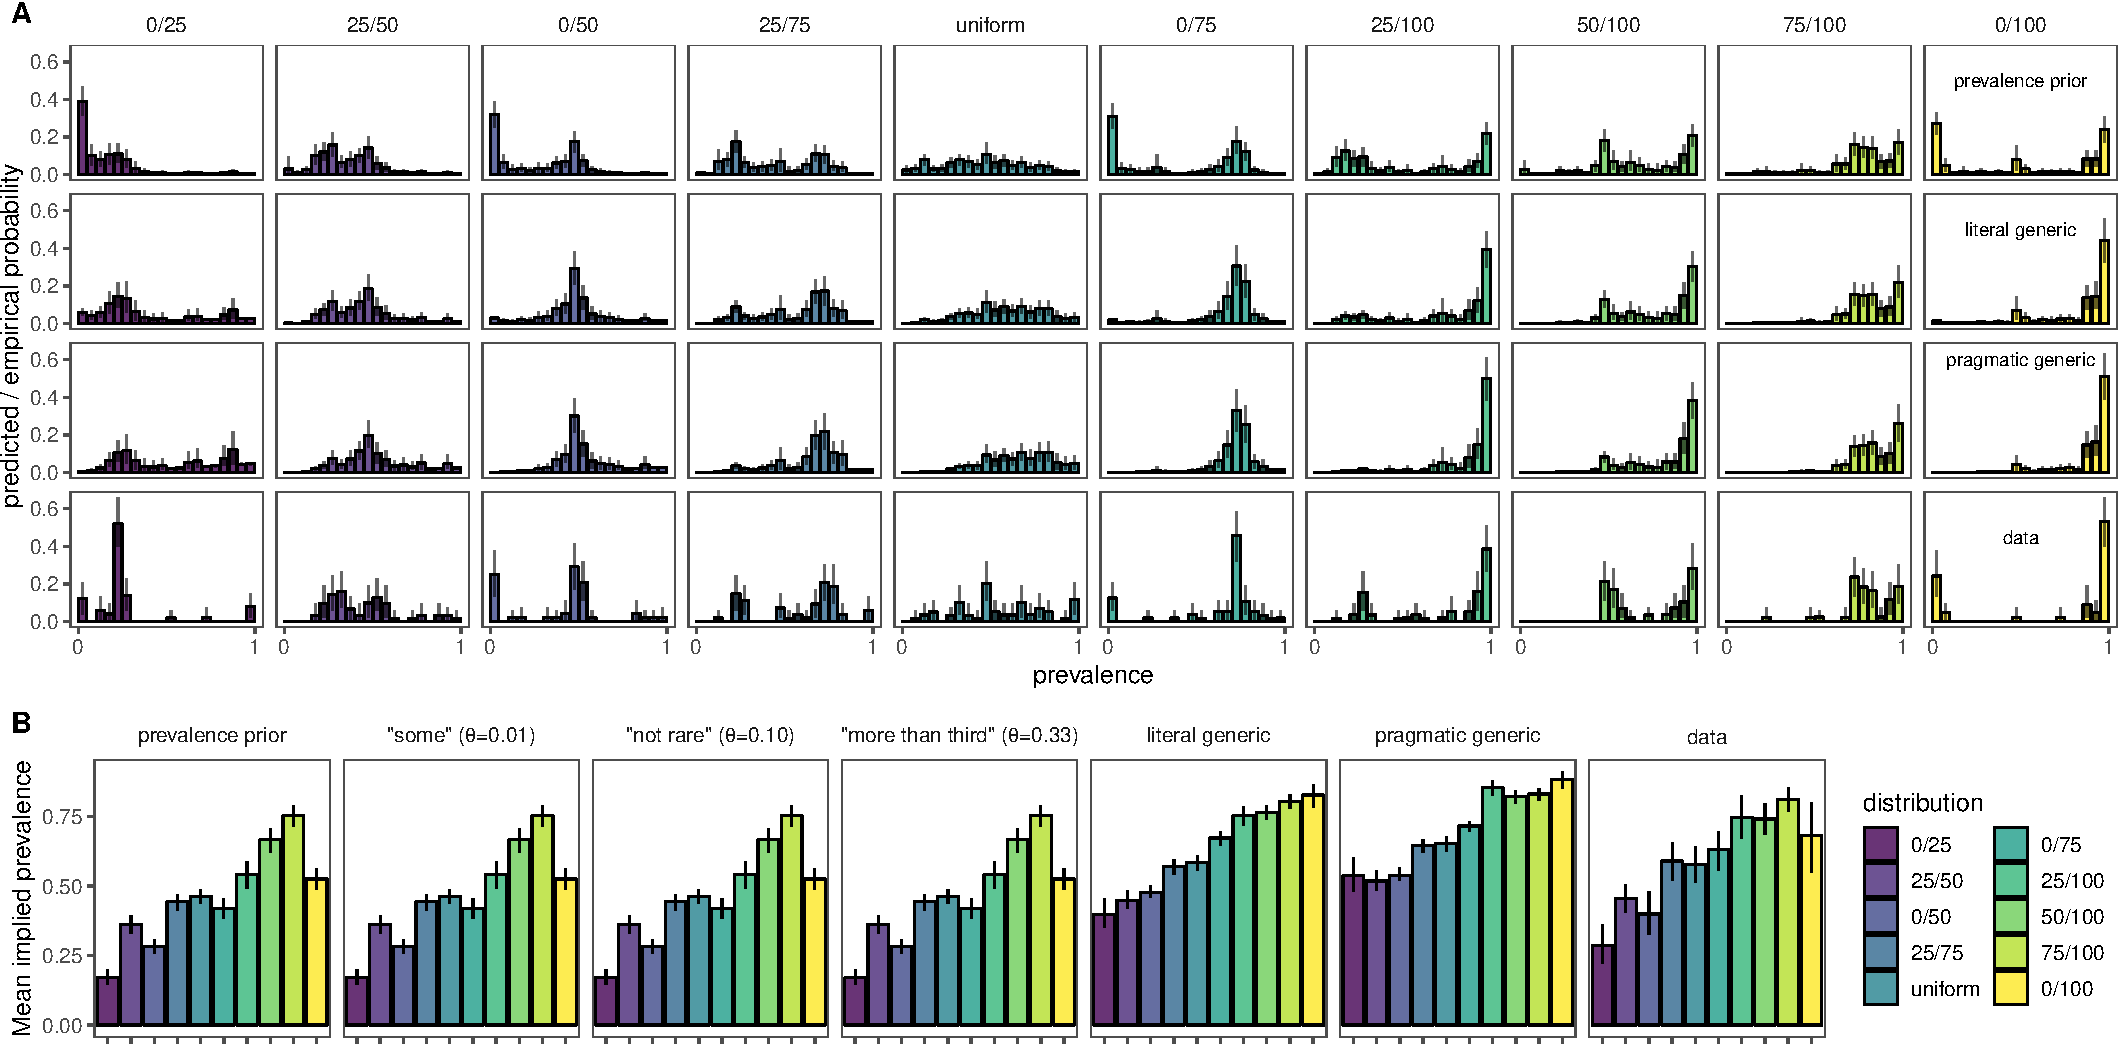
\includegraphics{genint_files/figure-latex/priorManipulationResults-1.pdf}
\caption{\label{fig:priorManipulationResults}Experiment 2 results. A: Empirical distribution of responses for the prior elicitation task (Expt. 2a), literal and pragmatic generics model predictions based on those empirical distributions, and empirical distributions of responses for the generic interpretation task (Expt. 3b). B: Model predicted means for alternative models and empirical means.}
\end{figure}

\hypertarget{results-2}{%
\subsubsection{Results}\label{results-2}}

We used preregistered exclusion criteria, which were also used for Expt. 2a.
Participants who failed to either select the correct property or list a correct number from the familiarization period were excluded (\(n = 39\)).
In addition, we excluded participants who self-reported a native language other than English (\(n = 33\)).
This left a total of \(n = 532\) participants, with items receiving on average 53 responses (range = {[}43, 62{]}).

Our main qualitative hypothesis is that there would be a difference across conditions in interpretations of the same generic sentence (\enquote{Ks know when earthquakes are about to happen}).
The differences in interpretations are visually evident in the empirical distributions of responses (Figure \ref{fig:priorManipulationResults}A, bottom row).
More specifically, we predict that the prevalence implied by the generic sentence will, to a first approximation, track the mean of the prevalence prior distribution.
To test this, we ran a linear model predicting responses with a fixed effect of the prior mean (as estimated by the data from Expt. 2a).
There was a significant main effect of prior mean, with a coefficient close to 1 (\(\beta_1 = 0.94\), \(SE=0.07\), \(t = 12.76\)), indicating a strong linear relationship between the mean of the learned prevalence prior and the resulting interpretations.
Furthermore, there was a significant main effect of intercept, indicating that participants' responses were significantly greater than the mean of the corresponding prevalence priors (\(\beta_0 = 0.16\), \(SE=0.04\), \(t = 4.44\)).
These results show that participants interpret the novel generic sentence in a manner sensitive to the background distribution and that the generic utterance updates participants' beliefs to indicate a prevalence significantly higher than the prior.
Still, there is much more to say about these data; this simple linear model explains less than a quarter of the variance in the data (\(r^2 = 0.24\)).

From the generics models, we are able to make a number of \emph{a priori} predictions about quantitative differences in mean implied prevalence ratings across the ten conditions.
These predictions were derived by examining pairs of conditions with small quantitative differences but for which the bootstrapped 95\% confidence interval around the generics model predictions did not overlap (Figure~\ref{fig:priorManipulationResults}B, \enquote{literal generic} panel).\footnote{These predictions were derived from the literal generic interpretation model. The experiment was planned before we developed the pragmatic generic interpretation model. Still, many of these predictions would have been derived from the pragmatic model following the same decision rule.}
With those criteria in mind, we preregistered the following contrast predictions among mean implied prevalences (\{\}s indicate no predicted difference): 0/25 \(<\) \{25/50, 0/50\} \(<\) \{25/75, \emph{uniform}\} \(<\) 25/75 \(<\) \{25/100, 50/100\} \(<\) \{75/100, 0/100\}.
To evaluate these predictions, we built a Bayesian regression model with the relevant contrasts using a \enquote{zero and one inflated beta} linking function to appropriately model the responses of exactly 0\% and 100\%, which are undefined under the beta distribution.
The maximum a-posteriori estimates and 95\% credible intervals of the coefficients of the regression model, as well as the model predicted qualitative differences, are shown in Table 2.
Each of the five predicted positive differences were estimated to be greater than zero, and each of the four predicted null differences were not different from zero.
Overall, the literal and pragmatic generic interpretation model predicts a lot of the variance in the means of these empirical distributions: (literal results: \(r^2(10) = 0.89; MSE = 0.00429\); pragmatic results: \(r^2(10) = 0.82; MSE = 0.0162\)).

\begin{table}[h]
\centering
\begingroup\fontsize{10pt}{11pt}\selectfont
\begin{tabular}{llrl}
  \hline
Coefficient & Prediction & Estimate & Credible Interval \\ 
  \hline
Intercept &  & 0.32 & [ 0.221, 0.418] \\ 
  0/25 vs. \{25/50, 0/50\} & $>$ & 0.15 & [ 0.036, 0.278] \\ 
  25/50 vs. 0/50 & = & -0.07 & [-0.270, 0.134] \\ 
  \{0/25, 25/50, 0/50\} vs. \{25/75, uniform\} & $>$ & 0.34 & [ 0.265, 0.409] \\ 
  25/75 vs. uniform & = & -0.00 & [-0.204, 0.189] \\ 
  \{25/75, uniform\} vs. 0/75 & $>$ & 1.14 & [ 0.903, 1.375] \\ 
  0/75 vs. \{25/100, 50/100\} & $>$ & 1.11 & [ 0.866, 1.352] \\ 
  25/50 vs. 50/100 & = & -0.09 & [-0.297, 0.127] \\ 
  \{25/100, 50/100\} vs. \{75/100, 0/100\} & $>$ & 0.52 & [ 0.307, 0.743] \\ 
  75/100 vs. 0/100 & = & -0.21 & [-0.458, 0.035] \\ 
   \hline
\end{tabular}
\endgroup
\caption{Regression model fits for planned comparisons. Predictions are based on whether the 95\% credible intervals for the generics model prediction overlap.} 
\end{table}

The computational models we articulate do more than just predict the \emph{mean} implied prevalence; they predict the full distribution of responses.
Again recall for this analysis, there are no free parameters in any of these models.
The model fits in terms of variance-explained and mean squared errors for the full distribution of responses are shown in Table 3.
To quantitatively compare the models in their ability to predict the empirical distributions of responses for these ten different conditions, we computed the likelihood of the data under each model by discretizing the empirical distributions and model predictions into ten equally spaced bins.
As is evident from Figure~\ref{fig:priorManipulationResults}A (bottom row, \enquote{data}), however, a number of participants responded that 0\% of Ks knew when earthquakes were about to happen when they read \enquote{Ks know when earthquakes are about to happen}.
Examining these participants' explanations revealed that the majority of these respondents believed they were answering a slightly different question than the one being asked; they believed they were responding to a question like in the prior elicitation task: Predict the next animal.
These \enquote{prior-type} responses are a source of noise in the data and one that affects all models (except the prior only model) to an equal degree.
All of the models we articulate have no way to account for 0\% responses, which are literally impossible given the utterance of the form \enquote{Ks F}.
To compute the likelihood of the complete data set under these models, we make the further assumption that the true generative process of the data is a mixture of responding according to one of the generic interpretation models and responding according to the prior.
We calculate Bayes Factors assuming a uniform distribution of noise between 0-20\% (approximated using the following discretization \(= \{0.001, 0.01, 0.05, 0.1, 0.15, 0.20\}\)).
To account for uncertainty in the measurement of the prior, we again bootstrap the model predictions by resampling the prior.
As is shown in Table 3, both the literal and pragmatic generic interpretation models are the best at predicting these data.
Because this experiment was designed to test the causal influence of the prevalence priors and not directly to compare these two models, the data do not definitively distinguish these two models from each other, owing to the relatively small differences in overall predictions for the two experimental conditions.
We conclude that the prevalence prior is causally related to interpretations of novel generics in the way predicted by the generics models.

\begin{table}[h]
\centering
\begingroup\fontsize{9pt}{10pt}\selectfont
\begin{tabular}{llll}
  \hline
Model & log Bayes Factor & expected value statistics & full distribution statistics \\ 
  \hline
Prior & -53.9 (-44, -63.6) & r\textsuperscript{2}(10) = 0.91; MSE = 0.0192 & r\textsuperscript{2}(200) = 0.49; MSE = 0.00381 \\ 
  Threshold = 0.01 & -48.6 (-39, -58.4) & r\textsuperscript{2}(10) = 0.83; MSE = 0.00887 & r\textsuperscript{2}(200) = 0.53; MSE = 0.00358 \\ 
  Threshold = 0.1 & -26.4 (-17.9, -35.4) & r\textsuperscript{2}(10) = 0.76; MSE = 0.00865 & r\textsuperscript{2}(200) = 0.56; MSE = 0.00334 \\ 
  Threshold = 0.35 & -48.6 (-39.3, -57.9) & r\textsuperscript{2}(10) = 0.7; MSE = 0.0114 & r\textsuperscript{2}(200) = 0.39; MSE = 0.00485 \\ 
  Literal Generic & 0 & r\textsuperscript{2}(10) = 0.89; MSE = 0.00429 & r\textsuperscript{2}(200) = 0.64; MSE = 0.00275 \\ 
  Pragmatic Generic & -2.1 (1.5, -5.6) & r\textsuperscript{2}(10) = 0.82; MSE = 0.0162 & r\textsuperscript{2}(200) = 0.55; MSE = 0.00352 \\ 
   \hline
\end{tabular}
\endgroup
\caption{Summary statistics for alternative generic interpretations. (Log) Bayes Factors quantify evidence in favor of each model in comparison to the uncertain threshold generics model. Numbers less than 0 indicate evidence in favor of the uncertain threshold model. Summary statistics displayed for the model fits for the expected values (means) of the distributions and the full (discretized) distributions.} 
\end{table}

\hypertarget{general-discussion}{%
\section{General Discussion}\label{general-discussion}}


%\red{SOcial import, minimal example (property)
%L0: predicate observed, all other features missing
%language is hard for actually describing specifics
%think about hte law
%good for minimal examples
%}

Generic language is the foremost case study of how abstract, generalizable knowledge is transmitted through language.
%, and it is commonly believed that generics carry strong interpretations (analogous to the quantifier \enquote{most} or \enquote{all}).
Despite their ubiquity and relative morphosyntactic simplicity, generics have been examined by few quantitative studies and no quantitative models that make predictions about how generic language updates beliefs.
Here, we explored the hypothesis that a generic statement can be literally thought of as conveying a single, minimal example to a listener.
This model is mathematically equivalent to the interpretation model assumed by Tessler \& Goodman (2019) where the generic acts a vague quantifier (Appendix A) and we articulated a more elaborate model which understands generics as intentional utterances.
We tested the models using a diverse set of stimuli and showed that the generic interpretations can be predicted with high-quantitative accuracy as a function of background knowledge about the property (Expt. 1).
Furthermore, we found that this background knowledge was causally responsible for the resulting interpretation (Expt. 2).
Finally, our data strongly support the conclusion that generics can be thought of as conveying a communicatively relevant minimal example as opposed to just literally a single observation. 
% interprets generics pragmatically provides a better explanation of the observed data than a literal interpretation model.
This work, thus, provides the computational formalism necessary to describe how beliefs are updated from generic language.

In the psychological literature on generics, generics are often thought of as conveying strong meanings.
The experimental data we present, however, shows that generics can receive a spectrum of interpretations, including being interpreted as only applying to a minority of the category (\emph{weak generics}). 
Statements like \enquote{Lorches live in zoos}, \enquote{Feps perform in the circus}, and \enquote{Wugs have seizures} all received average implied prevalence ratings below 50\%, with many individual participants providing ratings of 10\% or less (Expt. 1b).
When manipulating the prevalence prior distributions to suggest only prevalence levels of around 0\% or around 25\%, participants readily interpret the statement \enquote{Ks know when earthquakes are about to happen} to mean about 25\% (Expt. 2b).
This is an aspect of generic language understanding often swept under the rug: Generics are believed (in a generic sense) to carry strong implications.
Here, we show that generics also carry weak implications and all shades in-between.

\subsection{A communicatively relevant, minimal example}

The pragmatic generic interpretation model interprets a generic as conveying a communicatively relevant, minimal example to the listener. 
The example is minimal in the sense that the language picks out the correct feature for the listener to attend to and generalize. 
Drawing the same generalization from actual observational data alone would require significant covariation data to single out the feature relevant for generalization. 
Thus,  under this account, using generics for conveying generalizations is still expected to be more efficient than bonafide observational data because the speaker isolates a feature for generalization. 
Generics are also more useful than observations because speakers can describe properties that listeners could not in principle observe (Harris and Koenig, 2006). 

%The fact that the literal meaning of a generic is equivalent to observing a single positive instance of the category with a property suggests a very primitive foundation to generic language.
%Bayesian belief-updating based on observations is a general learning mechanism for any animal {\textcolor{Red}{(is there some citation for bayes in other animals?)}}.
%The work here suggests that the human unique component of understanding generic language comes not from understanding
%syntax or the meaning of the words but from understanding the communicative intent of the speaker {\textcolor{Red}{(cite tomasello?)}}.
The view of generics as communicatively relevant examples has been suggested by Csibra and Shamsudheen (2015), who argue that individual objects are interpreted by infants as symbolic representations of the object kind.
Under their account, a pedagogically presented exemplar from a category can be interpreted as a \enquote{nonverbal generic} by providing indexical reference to the object category.
The connection between generics and indexicality has also been made by Sterken (2015), who argues that the context-sensitivity exhibited by indexicals is the exact kind we need to model generics.
The model we present that interprets generics as communicatively relevant minimal examples is a very natural formalization of the nonverbal generic / indexical view.\footnote{
	One difference between our model and the view of Csibra and Shamsudheen (2015) is that our model does not assume any qualitative distinctions between ``generic knowledge'' and ``probabilistic knowledge''. All the knowledge in our model is probabilistic knowledge. 
	}


It may be surprising that our model for the semantics of generics as a single, minimal example is distinct from a model of existential quantification (i.e., the ``some'' model). 
After all, observing a single example of category with a property entails that at least one member of the category has the property. 
%The difference between existential quantification and a minimal example is that 
A minimal example is a more powerful belief-updating mechanism, however; in a sense, it is more concrete. 
Consider the case of trying to infer the weight of a biased coin: The quantifier ``some'' ($r > 0$) is tantamount to learning that it is not the case that both sides are tails; observing a minimal example requires actually flipping the coin and seeing it land on heads. 
Even without strong prior knowledge about the weight of a coin, it is more likely than not that the coin has a heads bias after observing just a single heads outcome; in fact, the most likely state of affairs to produce a single heads outcome (given uniform uncertainty about the weight of a coin) is that both sides of the coin are heads.
A minimal example entails existential quantification, but Bayesian reasoning updates beliefs based on an example in a stronger way.
Such a strong generalization is not supported by existential quantification.
\mht{anything to say about demonstratives like ``this fep has wings''?}

In our experiments, we investigate bare plural sentences, which are a common syntactic way of conveying generics (Gelman et al., 2008).
Generic meanings , however, can be packaged into different syntactic frames in English (e.g., ``A raven is black''; ``The blue-breasted quail eats small bugs and various grasses''), which are also commonly used to express concrete specifics (e.g., definite and indefinite singulars). 
Our ``minimal example'' semantics has a very natural analog to the semantics of an indefinite or definite singular.
The main difference is that with concrete reference, a speaker is referring to an instance that the listener knows about or could observe. 
Future work will need to investigate whether this formulation of the semantics of generics is sufficient to extend to generic meanings expressed in different syntactic frames. 

\hypertarget{the-relationship-between-prevalence-priors-and-generic-interpretations}{%
\subsection{The relationship between prevalence priors and generic interpretations}\label{the-relationship-between-prevalence-priors-and-generic-interpretations}}

{\textcolor{Green}{[ndg: people may worry about circularity of argument, given rich background knowledge elicitation that also uses language (similar to ellen's point). i think we should discuss this directly. relatedly we should discuss the implications of our structured background knowledge (elicitation and results).]}}
{\textcolor{Blue}{[mht: does this address it?]}}

In our experiments, we predict participants' implied prevalence ratings as a function of our computational model and empirical measurements about participants' background knowledge about properties. 
%The background knowledge elicitation tasks involve reasoning about the properties of alternative categories of animals.
%In order to elicit this knowledge, however, we conveyed instructions and questions using language. 
%Thus, there is the potential for circularity in our argument: We are predicting beliefs updated from language via beliefs elicited from language.
%A close inspection of the prior elicitation questions and our control quantitative models argue against circularity, however. 
%Our argument is not circular, however, because of the nature of the prior elicitation questions and our control quantitative models, which we describe below.
In Expt. 1a, we elicited background knowledge by having participants generate different animal categories and then later rate prevalence for different properties for those animals.
Here enters the potential for circularity in our method of predicting beliefs updated from language (\emph{generic interpretation}; Expt.~1b) via beliefs elicited from language (\emph{prevalence prior}; Expt.~1a).

It is possible that participants answer the prevalence question (e.g., \enquote{What percentage of dogs develop phobias?}) by first asking themselves internally a generic question (\enquote{Do dogs develop phobias?}) and then rating their personal generic-interpreted prevalence if the answer to this question was yes (and rating 0\% prevalence if the answer to the generic question was no).
If this view, beliefs about the generic are representationally primary (as is thought in the case of \emph{generic beliefs}; Prasada, 2000) and prevalence estimates are derived by participants' generic knowledge. 
Furthermore, under this view, the generic interpretation task (Expt.~1b) reduces to simply reporting back the part of the prior distribution that was generated when participants answered \enquote{yes} to their internally-directed generic question (\enquote{Do dogs develop phobias?}).
The prevalence priors do not seem to be simply a mixture of two distributions, and we have modeled each distribution as a mixture of three distributions because they exhibit complex structure. 
Furthermore, if this were the strategy participants employed, the most accurate model for the generic interpretation data would be the existentially-quantified \enquote{some} model, which rules out the 0\% component of the distribution.
The ``some'' model consistently underpredicts the generic interpretation data supporting the idea that belief-updating from generics is more nuanced that simply fixing a \emph{generic belief} node to be true (cf., Prasada, 2000; Csibra and Shamsudheen, 2015).


%If this were the case, there are only two possibilities for participants' beliefs---the category either does or does not (generically) have the property---and the generic interpretation task 
%
%
%The fact that the \enquote{some} model consistently underpredicts the generic interpretation data argues against the circularity in our measurements of the prevalence prior and generic interpretations.

Similarly, the patterns of data we observe in our experiments are additionally unlikely to be identical to those obtained using the quantifier \enquote{Some} (i.e., \enquote{Some Ks have F}).
Though we did not empirically measure judgments given the existentially quantified statements, the alternative model that assumes a fixed-threshold at 0\%-prevalence provides insight into what should be expected for those data.\footnote{Recall the fixed-threshold models are \enquote{literal interpretation} models and do not compute scalar implicatures.}
In both of our experiments, we found that the \enquote{some} model provided too weak of interpretations, consistent with the intuition that generic statements convey stronger prevalence implications that the existential statement.

%A similar argument can be made for the structured elicitation task in Expt. 1a.
%In Expt. 1, we assumed a particular model of the prevalence prior (i.e., a mixture of Betas) and elicited participants' knowledge about the property using questions that we assumed tapped into this structure.
%One question concerned the probability that a kind would have 0\% prevalence of the feature (or, equivalently, the proportion of categories for whom the property is expected to be present at some non-zero level of prevalence) by asking \enquote{How likely is it that \emph{there is a K with F}?}
%Intuitively, the response to such a question should be that it is very likely for properties that exist in many categories (e.g., \emph{is female}) and very unlikely for properties that only exist in a few categories (e.g., \emph{has purple feathers}).
%The second question concerned the shape of the non-zero conditional distribution of prevalence; this was measured by asking \enquote{\emph{Suppose there is a K with F}, how many Ks do you think have F?}.
%This question measures the projectibility of the property given a single, positive exemplar.
%Thus, the predictions of the alternative, fixed-threshold \enquote{some} model (which rules out 0\% prevalence) for this experiment correspond to the inferences upon learning that \emph{at least one member of the category has the property}.
%In Expt. 1, we again find the generic interpretation data are distinct from those of the conditional, non-zero distribution of prevalence, as evidenced by the \enquote{some} model comparisons.
%The fact that we use this \enquote{single, positive observation} question to elicit prior knowledge may in fact have blurred the distinction between the literal and the pragmatic model, which is why we Expt. 2 was conducted.


%Another interesting question is whether the same pattern of data could arise from a bonafide pedagogically sampled observation (cf., Csibra \& Shamsudheen, 2015).
%Given the success of the pragmatic model, we suspect this is possible, provided the pedagogical example is a minimal example. 
%We also suspect, however, an interaction with the alternative actions available to the speaker or teacher.
%That is, we do not expect bonafide generic interpretations from pedagogical demonstrations when the speaker could have said a generic.
%Finally, it should be noted that many of the properties used in our experimental stimuli are not directly observable either due to the nature of the property (e.g., \enquote{transmit HIV}) or to the habituality of the predicate (e.g., \enquote{fly into building windows}).


\subsection{Implications for stereotype amplification}

\mht{these two paragraphs are somewhat disconnected. if you think it's worthwhile, i can merge them}

The fact that understanding generics relies heavily on background knowledge about properties provides a clear avenue for miscommunication or deceit when using and learning from generics.
Cimpian et al. (2010) provided evidence for an \emph{asymmetry} between the conditions that permit a speaker to assert a generic and the prevalence learned by the listener from that same statement. 
The situation arises when a speaker endorses a generic when the prevalence is quite low (see Tessler \& Goodman, 2019) believing that they and the listener share the background assumptions that the property is a low-prevalence property in general.
The extent to which a listener has a different set of assumptions of the distribution of the property will result in miscommunication.
For many properties, the difference in implied prevalence may be inconsequential.
For features of social categories, which have difficult-to-understand statistical properties \red{(is there something about how people misunderstand the distributions of properties within social categories?)}, the misalignment of background  beliefs can lead to the propagation of stereotypes.
In fact, we saw that the biggest differences between the literal interpretation model (which guides the predictions of the generic speaker model used in Tessler \& Goodman, 2019) and the pragmatic generic interpretation model occur when the distribution of the property is most uncertain.

%Adults flexibly use their causal knowledge of the world to restrict the interpretation of a generic statement to a reasonable population, as evidenced by their explanations (e.g., \enquote{I thought that there would be many more Dobles in the wild than in zoos}).
%At the same time, the communicative force of a generic encodes a pressure for higher prevalence interpretations (e.g., without strong prior knowledge, generics imply high prevalence).
%Thus, listeners who do not have the substantial prior knowledge to restrict an interpretation of generics to a weak interpretation (e.g., young children) might derive a high-prevalence interpretation and furthermore posit abstract relations that would make a high-prevalence interpretation more likely.
%For example, upon learning \enquote{Dobles live in zoos}, a naive learner might infer that there is something about Dobles that causes them to live in zoos (cf., Prasada, Khemlani, Leslie, \& Glucksberg, 2013).
%This is potentially problematic for language about social categories (e.g., \enquote{Tall people are good at basketball}) for which an adult speaker might wish to convey a relatively low prevalence interpretation (e.g., \emph{some tall people\ldots{}} because most people are not good at basketball) but which a naive listener might derive a higher prevalence interpretation.
%This points to an aspect of generic meaning that might differ between adults and children: Whether or not children understand weak generics.



%The fact that an underspecified quantifier semantics proposed by Tessler and Goodman (2019) is equivalent to an observation model provides a route to learning the truth-functional meanings of natural language expressions through analogy to a more general learning mechanism. 
%That is, an uncertain quantifier updates beliefs in exactly the same way as a single positive observation. 


%\mht{What is Leslie's ``default generalization'', then? A single pedagogical observation}

%\mht{what do the words in the generic do? they point to the features that are relevant in the observation, kind of analogous to a demonstrator exaggerating their actions when producing a demonstration. they also point to the category to generalize (though, the actual category to generalize may be a restricted class (e.g., ``cabs are yellow'' [NYC cabs])}

%\mht{generics come in diverse syntax (within and across languages). ``A dog barks'' literally means one dog barked. ``You see a dog, it barks'' has the same semantics as both a particular and a generic?}

\mht{Lassiter suggested threshold version, and suggested that it might be reasoned about by the pragmatic listener. The results from the lifted threshold version of this model were inconclusive and we omitted them for brevity}

%\mht{another model: $x^n$ semantics... probably computationally indistinguishable as well}

%\mht{why is a single positive observation model different than the ``some'' model? ``some'' just tells you that both sides of the coin are not tails. gen tells you that you flipped it and it came up heads...}




%In what follows, we elaborate the assumptions in our modeling framework, describe how conceptual knowledge can guide prevalence-based interpretations, discuss how our answer to the problem of generic interpretation can inform an answer to the parallel problem of \emph{generic identification}, and speculate about the implications for communicating weak generics.
%
{\textcolor{Green}{[ndg: i'm not so sure about including these following discussion sections. they seem like interesting but only thematically related, as apposed to being crucial to our story or responses to probably objections. i didn't comment / edit them yet -- let's first decide if they stay.]}}


\hypertarget{conceptual-generic-interpretations}{%
\subsection{Conceptual generic interpretations}\label{conceptual-generic-interpretations}}

In this paper, we tested a particular model of generic interpretation that uses a prior distribution over the prevalence of a feature across relevant categories and assumes the truth-functional meaning of the generic is an uncertain threshold on the prevalence.
The prevalence prior distributions, which we elicit from participants, are likely influenced by the conceptual knowledge of our participants.
For example, the prevalence priors over properties that have to do with reproduction (e.g., \emph{have menstrual cycles}, \emph{get erections}) are multi-modal with one mode around 50\%, clearly reflecting participants' biological knowledge that these properties are specific to one sex of the animal.
We thus predict that 4-year-olds, who lack significant biological knowledge (Carey, 1985), would derive different interpretations than adults from generics about these properties.

Consistent with the intuition that conceptual knowledge underlies prevalence judgments, participants appeal to domain knowledge in their explanations for low-prevalence ratings, revealing aspects of their intuitive theories which guide their judgments.
One participant wrote: \enquote{About half are females and females have menstrual cycles.}
Another: \enquote{I assumed that only a percentage of Moxes were female and young enough to have a menstrual cycle.}
A typical explanation of a participant's response to \emph{Dobles live in zoos} was \enquote{I thought that there would be many more Dobles in the wild than in zoos. This is true of most animals in zoos today}.
Here, it is clear that the participant is using their knowledge of the property, derived from other animals, to learn about the category.
Participants often wrote about the lack of an enabling causal situation when describing their weak interpretations: \enquote{Most frams don't have access to nicotine.}
Explicitly modeling the intuitive theories that give rise to the intuitions about prevalence is an obvious future direction of this work.

Other semantic theories of generics make use of a mechanism by which the domain over which the prevalence of the feature in the category is calculated is contextually restricted (e.g., Cohen, 1999; Declerck, 1991).
In such a theory, the statement \enquote{Morseths have a menstrual cycle} gets evaluated as \enquote{Female morseths have a menstrual cycle}; under such an account, the implied prevalence of the feature would be 100\% (or near 100\%) because 100\% of the \emph{relevant lorches} (i.e., the females) have a menstrual cycle.\footnote{The scientifically correct term for a \enquote{menstrual cycle} is actually an \enquote{estrous cycle}. We are grateful to one of our MTurk participants for pointing this out to us. }
Interestingly, domain restricted interpretations are present in the empirical data.
Several properties about the reproductive behavior of animals (Expt. 1b) have interpretation distributions that are bimodal.
For example, \enquote{Morseths have a menstrual cycle} is interpreted primarily as applying to 50\% of morseths (38 out of 64 give a response between 45\% and 55\%); however, some participants (10 of 64) rate this as applying to 100\% of morseths.
This behavior could result from a participant interpreting the question as pragmatically restricting the domain to only the members of that category that \emph{could} have the property (e.g., 100\% of female morseths have a menstrual cycle).
The domain restricted interpretation is not limited to the generic interpretation data, however.
The bimodality is present in our prevalence elicitation task (Expt. 1a) as well: The distribution over several of the reproductive properties is tri-modal, with peaks at 0\% (the animals that don't have a menstrual cycle), 50\% (\enquote{only females}) and 100\% (perhaps, \enquote{all females}).
The fact that this multi-modality appears in the prior elicitation task means that the generic interpretation model predicts bi-modal interpretation distributions for the implied prevalence data, which is what we observe.
Still, the question remains why some participants interpret the noun phrase in generic statements as restricted to a salient subset of the category.

%\hypertarget{generic-identification}{%
%\subsection{Generic identification}\label{generic-identification}}
%
%{\textcolor{Blue}{[mht: i think this should be cut... unless you think there is something here?]}}
%
%Though often interpreted as generics, bare plural sentences (e.g., \enquote{Dogs bark}) can also manifest as \emph{non-generics} (e.g., \enquote{Dogs are on my front lawn}).
%Figuring out when a sentence expresses a generic meaning vs.~a non-generic meaning is called the problem of generic identification and is a parallel challenge to the problem of generic meaning (Carlson \& Pelletier, 1995).
%Our answer to the question \enquote{what do generics mean?} involves vagueness concerning the prevalence, which recruits beliefs about the property in question.
%The properties themselves may involve vagueness in terms of genericity, or its event counterpart \emph{habituality}, such as \emph{barks}: How often does an individual dog need to bark in order to qualify as a thing that barks?
%Tessler and Goodman (2019) showed that the same uncertain threshold mechanism explains graded endorsements of habitual statements like \enquote{John's dog barks}.
%
%The habituality of the predicate may actually be the source of the perceived generic/non-generic distinction.
%For instance, \enquote{Dogs are on my front lawn} exhibits only a single generalization (e.g., over \emph{dogs}); it is not a habitual predicate like \emph{barks}.
%The habituality of the predicate may influence the expected prevalence in the head noun category: A more vague, habitual predicate may be applied by human observers to more instances of the category because it is harder to verify than static properties.
%For non-habitual predicates, the expected prevalence would be substantially more restricted.
%Thus, we may find continuity in interpretations of underspecified noun phrases, including so-called \enquote{non-generics}: \enquote{Tigers have stripes} has higher implied prevalence than \enquote{Tigers are in the savanna} which is higher than \enquote{Tigers are in zoos}, \enquote{Tigers are in my local zoo}, and \enquote{Tigers are on my front lawn}.
%An uncertain threshold mechanism of the kind we have posited here may be such a way as to pragmatically infer a continuum of interpretations, from generics that are interpreted as universals (\enquote{Tigers are mammals}) to those that are interpreted existentially but habitually (\enquote{Tigers are in zoos}) to those that are interpreted existentially and non-habitually (\enquote{Tigers are on my front lawn}).
%Deriving such a prediction would necessarily involve a model of compositional generic interpretation, in which a habitual predicate meaning can be resolved jointly with a generic subject.


\hypertarget{conclusion}{%
\subsection{Conclusion}\label{conclusion}}

An easy way to acquire abstract knowledge is to understand a novel generic statement produced by a helpful interlocutor, but heretofore no quantitative models have accounted for how learning should occur from generic language.
 A computational model that understands generics as conveying communicatively relevant observations is able to predict the large variability in generic interpretations, even predicting the existence of \enquote{weak generics}, or generics that only apply to a minority of the category.
This work opens the door to understanding more precisely how abstract knowledge is learned from language.

\newpage

\hypertarget{references}{%
\section{References}\label{references}}

\hypertarget{refs}{}
\leavevmode\hypertarget{ref-Abelson1966}{}%
Abelson, R. P., \& Kanouse, D. E. (1966). Subjective acceptance of verbal generalizations. In S. Feldman (Ed.), \emph{Cognitive consistency: Motivational antecedents and behavioral consequents} (pp. 171--197). Academic Press.

\leavevmode\hypertarget{ref-Baker2009}{}%
Baker, C. L., Saxe, R., \& Tenenbaum, J. B. (2009). Action understanding as inverse planning. \emph{Cognition}, \emph{113}, 329--349. doi:\href{https://doi.org/10.1016/j.cognition.2009.07.005}{10.1016/j.cognition.2009.07.005}

\leavevmode\hypertarget{ref-carey1985conceptual}{}%
Carey, S. (1985). Conceptual change in childhood.

\leavevmode\hypertarget{ref-Carlson1977}{}%
Carlson, G. N. (1977). \emph{Reference to kinds in english} (PhD thesis). University of Massachusetts, Amherst.

\leavevmode\hypertarget{ref-Carlson1995}{}%
Carlson, G. N., \& Pelletier, F. J. (1995). \emph{The generic book.} Chicago, IL: Chicago University Press.

\leavevmode\hypertarget{ref-Cimpian2010}{}%
Cimpian, A., Brandone, A. C., \& Gelman, S. A. (2010). Generic statements require little evidence for acceptance but have powerful implications. \emph{Cognitive Science}, \emph{34}(8), 1452--1482.

\leavevmode\hypertarget{ref-Cimpian2009:explanations}{}%
Cimpian, A., \& Markman, E. M. (2009). Information learned from generic language becomes central to children's biological concepts: Evidence from their open-ended explanations. \emph{Cognition}, \emph{113}(1), 14--25. doi:\href{https://doi.org/10.1016/j.cognition.2009.07.004}{10.1016/j.cognition.2009.07.004}

\leavevmode\hypertarget{ref-Clark1996}{}%
Clark, H. H. (1996). \emph{Using language}. Cambridge University Press.

\leavevmode\hypertarget{ref-Cohen1999}{}%
Cohen, A. (1999). Generics, Frequency Adverbs, and Probability. \emph{Linguistics and Philosophy}, \emph{22}.

\leavevmode\hypertarget{ref-Csibra2015}{}%
Csibra, G., \& Shamsudheen, R. (2015). Nonverbal Generics: Human Infants Interpret Objects as Symbols of Object Kinds. \emph{Annual Review of Psychology}, \emph{66}, 689--710. doi:\href{https://doi.org/10.1146/annurev-psych-010814-015232}{10.1146/annurev-psych-010814-015232}

\leavevmode\hypertarget{ref-Declerck1991}{}%
Declerck, R. (1991). The origins of genericity. \emph{Linguistics}, \emph{29}, 79--102.

\leavevmode\hypertarget{ref-Frank2012}{}%
Frank, M. C., \& Goodman, N. D. (2012). Predicting pragmatic reasoning in language games. \emph{Science}, \emph{336}(6084).

\leavevmode\hypertarget{ref-Gelman2004}{}%
Gelman, S. A. (2004). Learning words for kinds: Generic noun phrases in acquisition. In \emph{Weaving a lexicon} (pp. 445--484). MIT Press.

\leavevmode\hypertarget{ref-Gelman2009}{}%
Gelman, S. A. (2009). Learning from others: Children's construction of concepts. \emph{Annual Review of Psychology}, \emph{60}, 115--140. doi:\href{https://doi.org/10.1146/annurev.psych.59.103006.093659.LEARNING}{10.1146/annurev.psych.59.103006.093659.LEARNING}

\leavevmode\hypertarget{ref-Gelman1998}{}%
Gelman, S. A., Coley, J. D., Rosengren, K. S., Hartman, E., \& Pappas, A. (1998). Beyond labeling: the role of maternal input in the acquisition of richly structured categories. \emph{Monographs of the Society for Research in Child Development}, \emph{63}(1), I--V, 1--148;discussion 149--157.

\leavevmode\hypertarget{ref-Gelman2008}{}%
Gelman, S. A., Goetz, P. J., Sarnecka, B. W., \& Flukes, J. (2008). Generic Language in Parent-Child Conversations. \emph{Language Learning and Development}, \emph{4}(1), 1--31. doi:\href{https://doi.org/10.1080/15475440701542625.Generic}{10.1080/15475440701542625.Generic}

\leavevmode\hypertarget{ref-Gelman2002}{}%
Gelman, S. A., Star, J. R., \& Flukes, J. E. (2002). Children's Use of Generics in Inductive Inferences. \emph{Journal of Cognition and Development}, \emph{3}(2), 179--199.

\leavevmode\hypertarget{ref-GelmanEtAl2004}{}%
Gelman, S. A., Taylor, M. G., Nguyen, S. P., Leaper, C., \& Bigler, R. S. (2004). Mother-child conversations about gender: Understanding the acquisition of essentialist beliefs. \emph{Monographs of the Society for Research in Child Development}, \emph{69}(1), vii, 116--127. doi:\href{https://doi.org/10.1111/j.1540-5834.2004.06901001.x}{10.1111/j.1540-5834.2004.06901001.x}

\leavevmode\hypertarget{ref-Goodman2016}{}%
Goodman, N. D., \& Frank, M. C. (2016). Pragmatic language interpretation as probabilistic inference. \emph{Trends in Cognitive Sciences}.

\leavevmode\hypertarget{ref-Goodman2013}{}%
Goodman, N. D., \& Stuhlmüller, A. (2013). Knowledge and implicature: Modeling language understanding as social cognition. \emph{Topics in Cognitive Science}.

\leavevmode\hypertarget{ref-dippl}{}%
Goodman, N. D., \& Stuhlmüller, A. (2014). The Design and Implementation of Probabilistic Programming Languages. \url{http://dippl.org}.

\leavevmode\hypertarget{ref-Grice1975}{}%
Grice, H. P. (1975). Logic and conversation. In \emph{Readings in language and mind}. Blackwell.

\leavevmode\hypertarget{ref-Khemlani2009}{}%
Khemlani, S., Leslie, S.-J., \& Glucksberg, S. (2009). Generics, prevalence, and default inferences. In \emph{Proceedings of the 31st annual conference of the cogntiive science society}. Austin, TX.

\leavevmode\hypertarget{ref-Khemlani2012}{}%
Khemlani, S., Leslie, S.-J., \& Glucksberg, S. (2012). Inferences about members of kinds: The generics hypothesis. \emph{Language and Cognitive Processes}, \emph{27}(6), 887--900. doi:\href{https://doi.org/10.1080/01690965.2011.601900}{10.1080/01690965.2011.601900}

\leavevmode\hypertarget{ref-LeeWagenmakers2014}{}%
Lee, M. D., \& Wagenmakers, E. (2014). \emph{Bayesian cognitive modeling: A practical course}. Cambridge: Cambridge University Press.

\leavevmode\hypertarget{ref-Leslie2008}{}%
Leslie, S.-J. (2008). Generics: Cognition and acquisition. \emph{Philosophical Review}, \emph{117}(1).

\leavevmode\hypertarget{ref-Levinson2000}{}%
Levinson, S. (2000). \emph{Presumptive meanings: The theory of generalized conversational implicature}. The MIT Press.

\leavevmode\hypertarget{ref-Montague1973}{}%
Montague, R. (1973). The Proper Treatment of Quantification in Ordinary English. In \emph{Philosophy, language, and artificial intelligence} (pp. 141-----162). Springer. Retrieved from \url{http://semantics.uchicago.edu/kennedy/classes/s08/semantics2/montague73.pdf}

\leavevmode\hypertarget{ref-neal2001annealed}{}%
Neal, R. M. (2001). Annealed importance sampling. \emph{Statistics and Computing}, \emph{11}(2), 125--139.

\leavevmode\hypertarget{ref-Prasada2013}{}%
Prasada, S., Khemlani, S., Leslie, S.-J., \& Glucksberg, S. (2013). Conceptual distinctions amongst generics. \emph{Cognition}, \emph{126}(3), 405--22. doi:\href{https://doi.org/10.1016/j.cognition.2012.11.010}{10.1016/j.cognition.2012.11.010}

\leavevmode\hypertarget{ref-Ritchie2016}{}%
Ritchie, D., Stuhlmüller, A., \& Goodman, N. D. (2016). C3: Lightweight incrementalized mcmc for probabilistic programs using continuations and callsite caching. In \emph{AISTATS 2016}.

\leavevmode\hypertarget{ref-hurdleModels}{}%
Rose, C. E., Martin, S. W., Wannemuehler, K. A., \& Plikaytis, B. D. (2006). On the use of zero-inflated and hurdle models for modeling vaccine adverse event count data. \emph{Journal of Biopharmaceutical Statistics}, \emph{16}(4), 463--481.

\leavevmode\hypertarget{ref-problang}{}%
Scontras, G., Tessler, M. H., \& Franke, M. (2018). Probabilistic language understanding: An introduction to the Rational Speech Act framework.

\leavevmode\hypertarget{ref-Shepard1987}{}%
Shepard, R. N. (1987). Toward a universal law of generalization for psychological science. \emph{Science (New York, N.Y.)}, \emph{237}(4820), 1317--1323. doi:\href{https://doi.org/10.1126/science.3629243}{10.1126/science.3629243}

\leavevmode\hypertarget{ref-Sterken2015}{}%
Sterken, R. K. (2015). Generics in Context. \emph{Philosophers' Imprint}, \emph{15}(i), 1--30.

\leavevmode\hypertarget{ref-Tenenbaum2011}{}%
Tenenbaum, J. B., Kemp, C., Griffiths, T. L., \& Goodman, N. D. (2011). How to grow a mind: statistics, structure, and abstraction. \emph{Science (New York, N.Y.)}, \emph{331}(6022), 1279--85. doi:\href{https://doi.org/10.1126/science.1192788}{10.1126/science.1192788}

\leavevmode\hypertarget{ref-Tessler2019psychrev}{}%
Tessler, M. H., \& Goodman, N. D. (2019). The language of generalization. \emph{Psychological Review}.

\newpage
\section{Appendix A: Equivalence to an uncertain threshold model}

Belief-updating based on a single positive observation is mathematically equivalent to the interpretation model proposed by Tessler and Goodman (2019), as belief-updating based on a threshold-function (e.g., \(\mbox{ $[\![ gen ]\!]$} = r > \theta\)) whose threshold value is uncertain and is drawn from a uniform prior (\(\theta \sim \text{Uniform}(0, 1)\)):

\begin{align}
L_0(r, \theta \mid u) \propto {\delta_{\mbox{ $[\![ u ]\!]$}(r, \theta)} \cdot P(r) \cdot P(\theta)} \label{eq:L0a}
\end{align}

Here, the truth-functional meaning of a generic is a threshold-function mandating that the prevalence \(r\) is greater than the threshold \(\theta\), represented by the Kronecker delta \(\delta_{\mbox{ $[\![ u ]\!]$}(r, \theta)}\) that returns \(1\) when the utterance is true (i.e., when \(r > \theta\)) and \(0\) otherwise.
%
%\begin{align}
%\delta_{\mbox{ $[\![ u_{gen} ]\!]$}(r, \theta)} &\propto  \begin{cases}
%1 & \text{if } r > \theta \\
%0 & \text{otherwise}
%\end{cases}\label{eq:delta}
%\end{align}
%
This version of the model uses the standard truth-functional tools of formal semantics (Montague, 1973) and relates to the literal semantics of quantifiers, which can also be described by threshold functions (e.g., \(\mbox{ $[\![ some ]\!]$} = r > 0\), \(\mbox{ $[\![ most ]\!]$} = r > 0.5\), \(\mbox{ $[\![ all ]\!]$} = r = 1\)).
Note that since \(\theta \sim \text{Uniform}(0, 1)\),  \(P(\theta) \propto 1\)  and thus Equation \ref{eq:L0a} can be rewritten as: \(L_0(r, \theta \mid u) \propto P(u \mid r, \theta)\) where

\begin{align}
P(u \mid r, \theta)  &\propto \begin{cases}
P(r) & \text{if } r > \theta \\
0 & \text{otherwise} \end{cases} \label{eq:delta2}
\end{align}

\noindent To arrive at \(L_0(r \mid u)\) from Equation \ref{eq:delta2}, we integrate out \(\theta\).

\begin{align}
L_0(r, \mid u) =& \int_{0}^{1} L_0(r, \theta \mid u) \mathop{}\!\mathrm{d}\theta \nonumber \\
\propto& \int_{0}^{1} P(u \mid r, \theta)  \mathop{}\!\mathrm{d}\theta \nonumber \\
=& \int_{0}^{r} P(u \mid r, \theta) \mathop{}\!\mathrm{d}\theta + \int_{r}^{1}P(u \mid r, \theta) \mathop{}\!\mathrm{d}\theta \nonumber \\
=& \int_{0}^{r} P(r) \mathop{}\!\mathrm{d}\theta + \int_{r}^{1} 0 \mathop{}\!\mathrm{d}\theta \nonumber  \\ 
   = &  P(r) \int_{0}^{r} \mathop{}\!\mathrm{d}\theta \nonumber \\
     = &   P(r) \cdot r \label{eq:L0d}
\end{align}

Thus, the model of Tessler and Goodman (2019) that assumes the literal meaning of a generic utterance is a uniformly uncertain threshold-function is mathematically equivalent to Bayesian belief-updating based on a single positive observation. 

\newpage
\hypertarget{appendix-items}{%
\section{Appendix B: Items}\label{appendix-items}}

\begingroup\fontsize{11pt}{12pt}\selectfont
\begin{longtable}{ |p{3in}|}
  \hline
{\bfseries Property} \\ 
  \hline
are afraid of dogs \\ 
   \hline
are afraid of loud noises \\ 
   \hline
are intelligent \\ 
   \hline
attack hikers \\ 
   \hline
attract mates by secreting pheromones \\ 
   \hline
cannibalize each other \\ 
   \hline
capture other animals territory \\ 
   \hline
carry Lyme disease \\ 
   \hline
carry malaria \\ 
   \hline
carry out premeditated murder \\ 
   \hline
chase their tails \\ 
   \hline
develop back problems \\ 
   \hline
develop phobias \\ 
   \hline
do handstands to scare off predators \\ 
   \hline
drink alcohol left behind by tourists \\ 
   \hline
drink soda \\ 
   \hline
eat candy wrappers \\ 
   \hline
eat cannabis \\ 
   \hline
eat garbage \\ 
   \hline
eat grass \\ 
   \hline
eat human food \\ 
   \hline
eat insects \\ 
   \hline
eat people \\ 
   \hline
experience emotions \\ 
   \hline
experience empathy \\ 
   \hline
feed on the carcasses of dead animals \\ 
   \hline
fish in the Hudson River \\ 
   \hline
fly into building windows \\ 
   \hline
get addicted to nicotine \\ 
   \hline
get cancer \\ 
   \hline
get dandruff \\ 
   \hline
get erections \\ 
   \hline
get in fights with other animals \\ 
   \hline
give birth underwater \\ 
   \hline
go bald \\ 
   \hline
have a menstrual cycle \\ 
   \hline
have an exquisite sense of smell \\ 
   \hline
have brown fur \\ 
   \hline
have dozens of sexual partners \\ 
   \hline
have four legs \\ 
   \hline
have intensely beautiful feathers \\ 
   \hline
have personalities \\ 
   \hline
have seizures \\ 
   \hline
have spots \\ 
   \hline
have strange genetic mutations \\ 
   \hline
have very long wings \\ 
   \hline
hunt other animals \\ 
   \hline
know how to open doors \\ 
   \hline
know how to ride bicycles \\ 
   \hline
know when earthquakes are about to happen \\ 
   \hline
lay eggs in other birds nests \\ 
   \hline
lay eggs without needing fertilization \\ 
   \hline
like to cuddle \\ 
   \hline
live in high-rise buildings \\ 
   \hline
live in the hulls of sea vessels \\ 
   \hline
live in trees \\ 
   \hline
live in urban areas \\ 
   \hline
live in zoos \\ 
   \hline
live to be a hundred years old \\ 
   \hline
live to be five hundred years old \\ 
   \hline
live to be twenty years old \\ 
   \hline
lose their teeth \\ 
   \hline
mourn their dead \\ 
   \hline
perform in the circus \\ 
   \hline
play with bottlecaps \\ 
   \hline
pound their chests to display dominance \\ 
   \hline
ride the subway \\ 
   \hline
sing beautiful songs \\ 
   \hline
sleep during the day \\ 
   \hline
steal farmers crops \\ 
   \hline
swim in shallow pools \\ 
   \hline
torture other animals \\ 
   \hline
transmit HIV \\ 
   \hline
transmit rabies \\ 
   \hline
use tools \\ 
   \hline
\hline
\caption{Items used in Expt. 1} 
\end{longtable}
\endgroup

\newpage


\end{document}
